\documentclass[12pt,a4paper, onecolumn]{exam}
\usepackage{amsmath}
\usepackage{amssymb}
\usepackage[lmargin=0.3in, rmargin=0.3in, top=0.3in, bottom=0.8in]{geometry}  %For centering solution box
\usepackage[shortlabels]{enumitem}
\usepackage{subcaption}
\usepackage[final]{graphicx}
\usepackage{float}
\usepackage{appendix}
\usepackage{titlesec}
% \lhead{Leaft Header\\}
% \rhead{Right Header\\}
% \chead{\hline} % Un-comment to draw line below header
% \thispagestyle{empty}   %For removing header/footer from page 1

\titlespacing*{\section}{0pt}{*0.5}{*0.5}
\titlespacing*{\subsection}{0pt}{*0.5}{*0.5}
\titlespacing*{\subsubsection}{0pt}{*0.5}{*0.5}
\titlespacing*{\paragraph}{0pt}{*0.5}{*0.5}
\expandafter\def\expandafter\normalsize\expandafter{%
    \normalsize%
    \setlength\abovedisplayskip{5pt}%
    \setlength\belowdisplayskip{5pt}%
    \setlength\abovedisplayshortskip{5pt}%
    \setlength\belowdisplayshortskip{5pt}%
}
\setlength{\textfloatsep}{0.5em}
\setlength{\floatsep}{0.5em}
\setlength{\intextsep}{0.5em}
\setlist[itemize]{itemsep=0pt, topsep=0pt}
\begin{document}

\begingroup
\centering
\LARGE Machine Learning: Project\\
\LARGE Multi-Agent Learning in Canonical Games and Knights Archers Zombies\\[0.5em]
\large \today\\[0.5em]
\large Dimitrios Mystriotis - Jan Cichomski\par
\large r1027781 - r1026448\par
\endgroup
\rule{\textwidth}{0.4pt}
\pointsdroppedatright   %Self-explanatory
\printanswers
\renewcommand{\solutiontitle}{\noindent\textbf{Ans:}\enspace}   %Replace "Ans:" with starting keyword in solution box
\section*{Source Code and Time Spent}
\textbf{Source Code} for part 1 and 2 is in: \texttt{/cw/lvs/NoCsBack/vakken/H0T25A/ml-project/r1026448}\\
\textbf{Time Spent} by Jan Cichomski (r1026448) around 80h, by Dimitrios Mystriotis (r1027781) around 80h.

\section{\textbf{Task 1:}}
% \subsection{TODOs}
% \begin{itemize}
%     \item make sure its max 10 pages
% read everything and make sure it is coherent
% pass it through Grammarly checker
% \end{itemize}

\subsection{Algorithmic, Game-Theoretic, and Logical Foundations}
This book \cite{shoham} defines the Nash Equilibrium as "A strategy profile $s = (s1,... ,sn)$ is a Nash equilibrium if, for all agents $i$, $s_i$ is a best response to $s_{-i}$." \cite{shoham}.
This means that all agents in the game are playing their best response to every other agent's strategy. The Nash Equilibrium is a stable state of the game, where no agent can improve their outcome by changing their strategy.

It is also split between Strict and Weak Nash Equilibrium, where a Nash Equilibrium is Strict if there is a unique strategy for every agent that provides the best outcome ($u_i(s_i, s_{-i}) > u_i(s'_i,s_{-i})$).
A Nash Equilibrium is Weak if multiple strategies provide the same outcome ($u_i(s_i, s_{-i}) \geq u_i(s'_i,s_{-i})$).

When trying to compute the Nash Equilibrium in a two-player, general-sum game like the ones in this project, the best way is to use the Lemke-Howson algorithm,
as this algorithm is "the best known algorithm for the two-player, general-sum case" \cite{shoham}.

Also, Pareto Optimality is defined as "Strategy profile $s$ is Pareto optimal, or strictly Pareto efficient, if there does not exist another strategy profile $s' \in S$ that Pareto dominates $s$." \cite{shoham}.
This means that there is no other strategy that can make one agent better off without making other agents worse off. Pareto Optimal solutions are the best possible solution for all agents in the game.
All games have at least one Pareto Optimal solution, but not all games have a pure strategy Nash Equilibrium.

\subsection{A Comprehensive Survey of Multiagent Reinforcement Learning}

From this paper \cite{busoniu}, we are interested mostly in the $\epsilon$-Greedy algorithm and the Boltzmann algorithm. These algorithms were implemented as described in the paper and tested on the canonical games.
$\epsilon$-Greedy is a simple algorithm that chooses the best action according to the greedy policy \ref{eq:egreedy} with probability $1 - \epsilon$ and a random action with probability $\epsilon$.
\begin{equation}\label{eq:egreedy}
    \bar{h}(x) = argmax_{a \in A} Q(x,a)
\end{equation}
where $Q(x,a)$ is the Q value of the action a in the state x, and A is the set of all possible actions.
Using a probability $\epsilon$ allows for exploration of the problem space and satisfies the requirement for convergence that the agent needs to keep trying all actions
in all states with nonzero probability.

The Boltzmann algorithm is a more complex algorithm that chooses the next action with probability
\begin{equation}\label{eq:boltzmann}
    P(a) = \frac{e^{Q(x,a)/\tau}}{\sum_{a' \in A} e^{Q(x,a')/\tau}}
\end{equation}
where $\tau$ is the temperature parameter. The Boltzmann algorithm is a stochastic algorithm that allows for exploration of the problem space. The temperature parameter $\tau$ is responsible
for the amount of exploration the algorithm will perform. A high $\tau$ value will make the algorithm explore more, while a low $\tau$ value will make the algorithm exploit more.

\subsection{Evolutionary Dynamics of Multi-Agent Learning: A Survey}

From this paper \cite{bloembergen}, we are interested in the Lenient Boltzmann algorithm. The Lenient Boltzmann algorithm is a modification of the Boltzmann algorithm that evaluates actions more optimistically.
This is done by letting the agent evaluate their action against K possible actions from the opponent and keeping the best reward. In this way, potential mistakes in the start of the training
are not punished as hard as in the Boltzmann algorithm.

Replicator dynamics are also explained in this paper. The replicator dynamics are a set of differential equations that describe the evolution of the population of strategies in a game.
Specifically, they model the change in the frequency of strategies in a population. This population can be described as a state vector $x = (x_1, x_2, ..., x_n)$ where $x_i$ is the frequency of
strategy i in the population. If the fitness of these strategies is given by the fitness function $f(x)$, the replicator dynamics are given by the equation
\begin{equation}\label{eq:replicator}
    \dot{x_i} = x_i(f_i(x) - \bar{f}(x))
\end{equation}
where $f_i(x)$ is the fitness of strategy i and $\bar{f}(x)$ is the average fitness of the population.

\section{\textbf{Task 2:}}
\subsection{Nash Equilibria and Pareto Optimality}

\begin{itemize}
    \item \textit{Stag Hunt:}
          The pure \textbf{Nash Equilibria} are (Hare, Hare) and (Stag, Stag), with a mixed strategy \textbf{Nash Equilibrium} also existing. % with each side picking (Stag, Hare) = (0.66,0.34).
          The \textbf{Pareto Optimal} strategy is (Stag, Stag).

    \item \textit{Subsidy Game:}
          The pure \textbf{Nash Equilibria} are (Subsidy 1, Subsidy 1) and (Subsidy 2, Subsidy 2), with a mixed strategy \textbf{Nash Equilibrium} also existing. %with each side picking (Subsidy 1, Subsidy 2) = (0.9091,0.0909).
          The \textbf{Pareto Optimal} strategy is (Subsidy 1, Subsidy 1).

    \item \textit{Matching Pennies:}
          There is no \textbf{Nash Equilibrium} for a pure strategy. For a mixed strategy, the \textbf{Nash Equilibrium} is picking heads or tails with probability 0.5 each \cite{shoham}.
          Every outcome is \textbf{Pareto Optimal}.

    \item \textit{Prisoner's Dilemma:}
          The pure \textbf{Nash Equilibrium} is (Defect, Defect).
          The \textbf{Pareto Optimal} strategy is (Cooperate, Cooperate).
\end{itemize}

\subsection{Learning Trajectories}
\subsubsection{$\epsilon$-Greedy Q-Learning}
The $\epsilon$-Greedy algorithm converges to the Nash Equilibrium for all games. Even when an algorithm converges to the Pareto Optimal solution, it moves towards the Nash Equilibrium
as the number of iterations increases. This is because the Nash Equilibrium is the most stable solution, which random choices will favor. For the learning trajectories of $\epsilon$-Greedy,
the action choice depends on Q values, and it is picked deterministically. This makes it complicated to plot the learning trajectories, as the probabilities of choosing an action are
constant, making it hard to plot a graph, so we plot the normalized Q-values instead. An example of a learning trajectory is shown in Fig. \ref{fig:greedy_combined}.

% The Q-values mean absolutely nothing on there own. We need a graph to compare Q for action 1 to Q for action 2.
\begin{figure}[h]
    \centering
    \begin{subfigure}{0.49\textwidth}
        \centering
        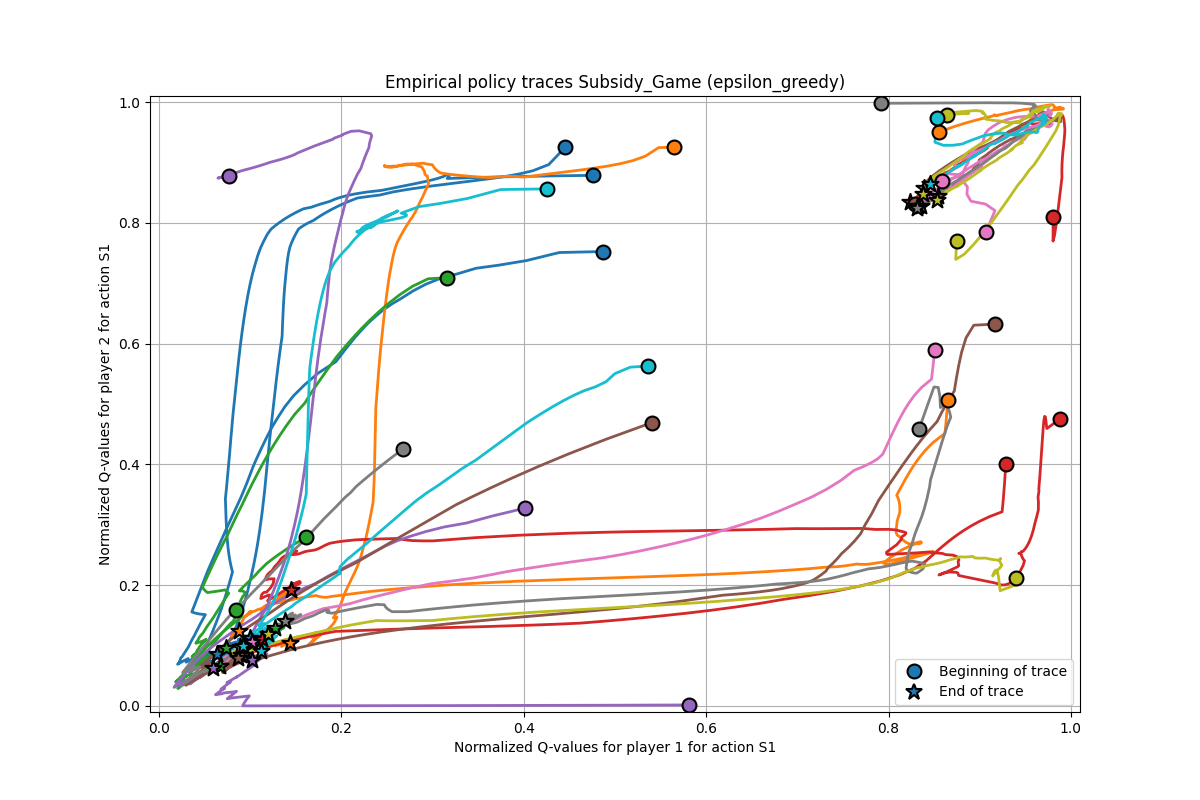
\includegraphics[width=\linewidth]{plots/replicator_trajectoreis_Subsidy_Game_epsilon_greedy.png}
        \caption{Subsidy Game}
        \label{fig:egsg}
    \end{subfigure}
    \hfill
    \begin{subfigure}{0.49\textwidth}
        \centering
        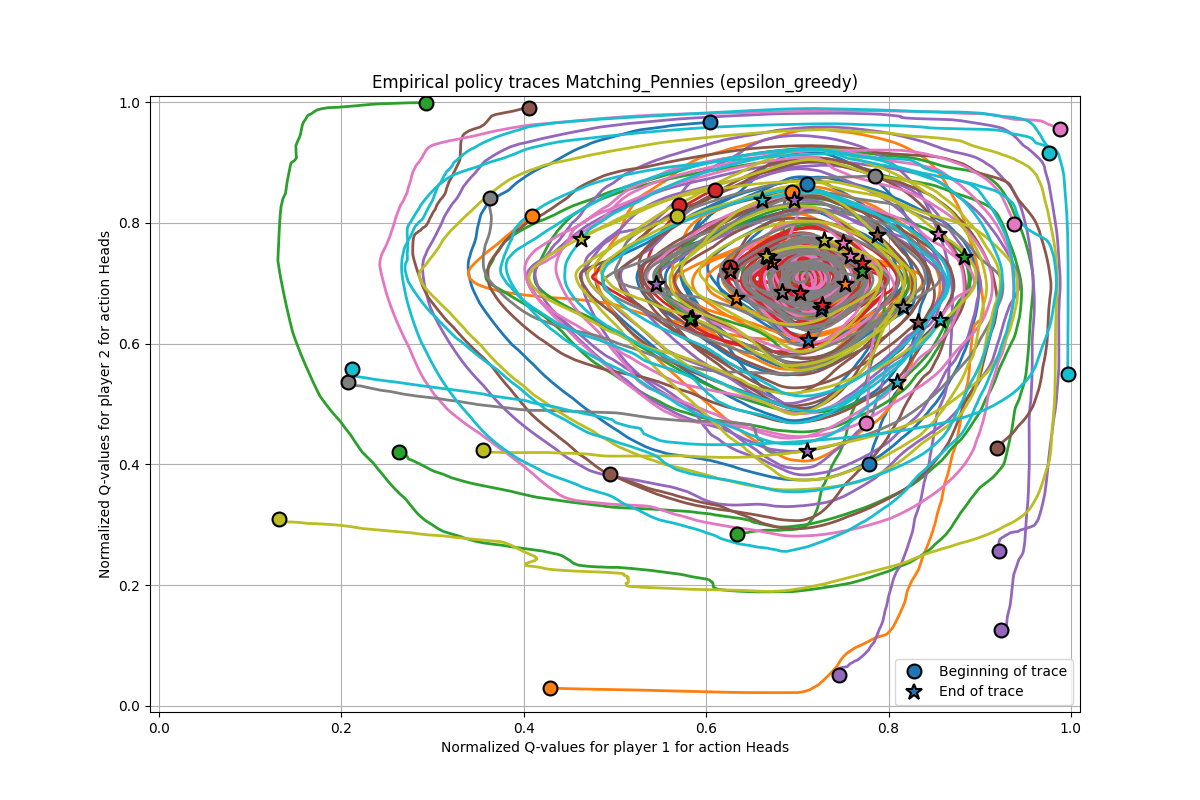
\includegraphics[width=\linewidth]{plots/replicator_trajectoreis_Matching_Pennies_epsilon_greedy.png}
        \caption{Matching Pennies}
        \label{fig:egpd}
    \end{subfigure}
    \caption{Empirical policy traces (normalized Q-values) for $\epsilon$-Greedy Q-Learning ($\epsilon=0.1$), (a) Subsidy Game and (b) Matching Pennies.}
    \label{fig:greedy_combined}
\end{figure}
\paragraph{Convergence Analysis ($\epsilon=0.1$, $lr=0.1$)}
We analyzed the convergence of $\epsilon$-Greedy Q-Learning regarding Nash Equilibria (NE) and Pareto Optimality (PO) across the games:

\begin{itemize}
    \item \textit{Stag Hunt:} Most traces converged to the (Hare, Hare) NE.
          Few traces starting near the (Stag, Stag) NE, which is also PO, converged there.
          Convergence to the PO solution was infrequent, likely due to insufficient exploration.
    \item \textit{Subsidy Game:} Most traces converged to (Subsidy 2, Subsidy 2),
          a NE but not PO. Some traces starting near the alternative NE and PO (Subsidy 1, Subsidy 1)
          converged there, possibly limited exploration preventing them from reaching the PO outcome.
    \item \textit{Matching Pennies:} All Traces converged towards (Heads, Heads) and oscillated around it.
          While this outcome is PO (as all are in this game), it is not an NE, which does not exist.
    \item \textit{Prisoner's Dilemma:} Most traces converged to the (Defect, Defect) NE.
          Only a minority reached the PO solution (Cooperate, Cooperate).
\end{itemize}

Overall, convergence was highly sensitive to initial conditions. Trajectories very rarely converge to the exact strategy suggested by the NE or the PO.
This indicates that $\epsilon=0.1$ provided some volatility in action selection, which would cause the algorithm to deviate from a 100\% certainty about
a strategy. This results from the $\epsilon$-Greedy algorithm's deterministic aspect, which means that it will always pick the action with the highest Q-value.
This converts what looks like a mixed strategy on the graph (Fig. \ref{fig:greedy_combined}) into a pure strategy with some extra randomness ($\epsilon$).

\subsubsection{Boltzmann Q-Learning} \label{sec:boltzmann}

The Boltzmann algorithm is a stochastic algorithm that allows for exploration of the problem space. Action selection is done probabilistically based on their Q-values.
The use of a temperature parameter $\tau$ is responsible for the exploration vs exploitation trade-off, making it very flexible for these kinds of problems.
An example of a learning trajectory is shown in Fig. \ref{fig:boltzmann_combined}.
\begin{figure}[h]
    \centering
    \begin{subfigure}{0.49\textwidth}
        \centering
        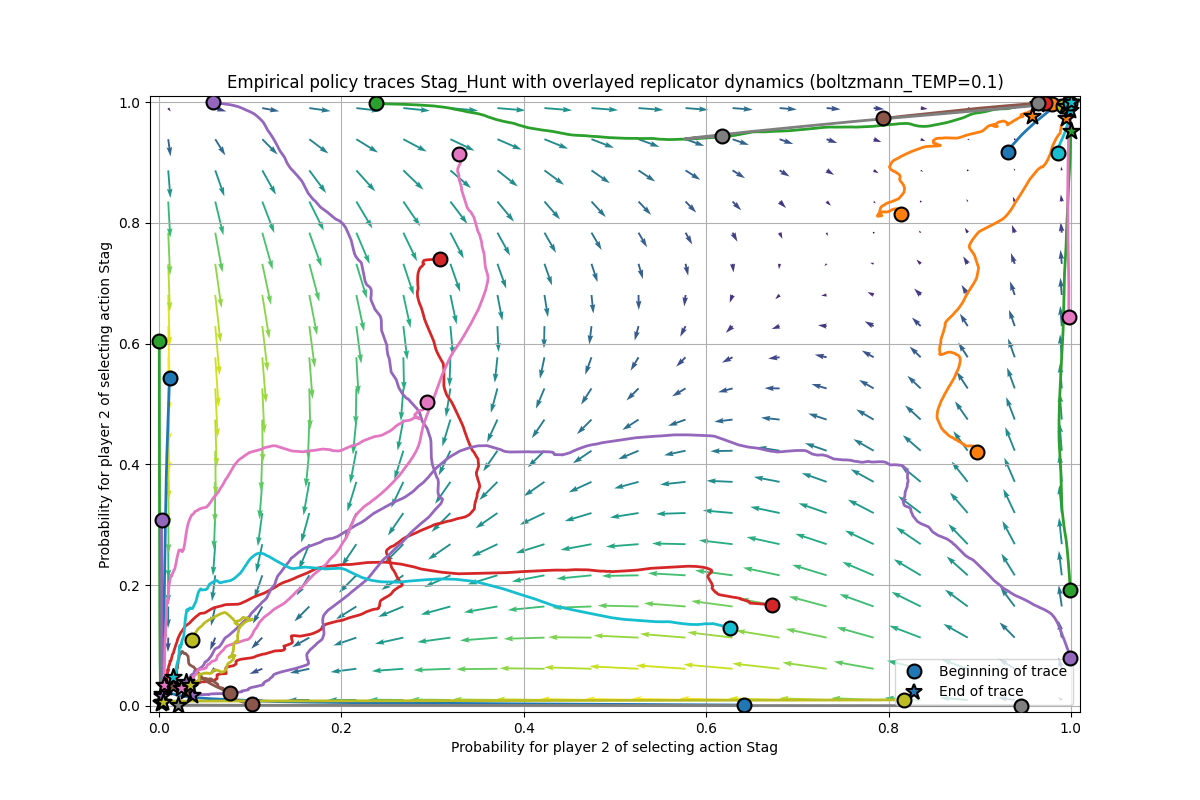
\includegraphics[width=\linewidth]{plots/replicator_trajectoreis_Stag_Hunt_boltzmann_TEMP=0.1.png}
        \caption{Stag Hunt}
        \label{fig:bsh}
    \end{subfigure}
    \hfill
    \begin{subfigure}{0.49\textwidth}
        \centering
        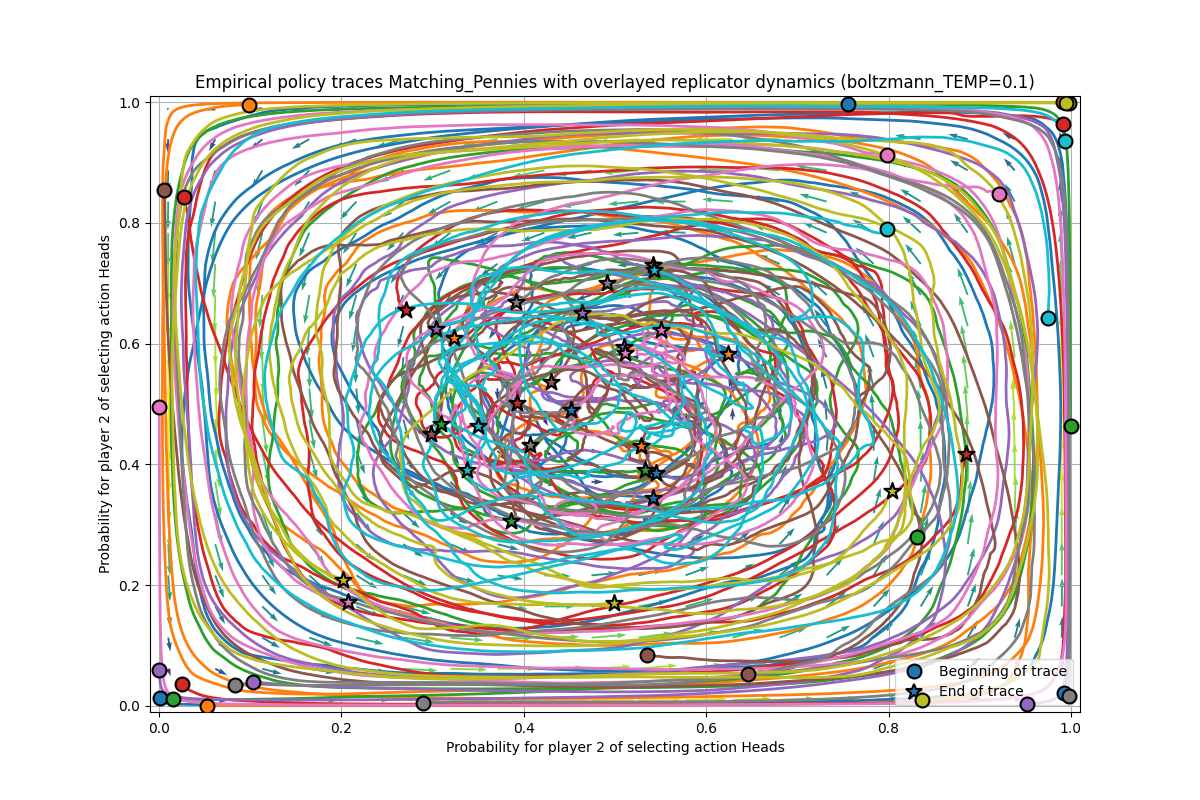
\includegraphics[width=\linewidth]{plots/replicator_trajectoreis_Matching_Pennies_boltzmann_TEMP=0.1.png}
        \caption{Matching Pennies}
        \label{fig:bmp}
    \end{subfigure}
    \caption{Empirical policy traces for Boltzmann Q-Learning (temperature = 0.1), (a) Stag Hunt and (b) Matching Pennies.}
    \label{fig:boltzmann_combined}
\end{figure}
\paragraph{Convergence Analysis (temperature=0.1, learning rate = 0.1)}
We analyzed the convergence of Boltzmann Q-Learning regarding Nash Equilibria (NE) and Pareto Optimality (PO):

\begin{itemize}
    \item \textit{Stag Hunt:} Traces converged to both NEs: (Hare, Hare) and (Stag, Stag).
          Convergence to the PO solution (Stag, Stag) was less frequent than the NE (Hare, Hare).
    \item \textit{Subsidy Game:} Most traces converged to the (Subsidy 2, Subsidy 2) NE, which is not PO.
          A few traces initialized near the (Subsidy 1, Subsidy 1) NE (which is PO) converged there instead.
    \item \textit{Matching Pennies:} Traces oscillated around a random strategy without converging to a pure strategy, consistent
          with the lack of a pure strategy NE (Fig. \ref{fig:bmp}). All outcomes in this game are PO.
    \item \textit{Prisoner's Dilemma:} Most traces converged to the (Defect, Defect) NE, which is not PO.
          Very few traces converged to the PO outcome (Cooperate, Cooperate).
\end{itemize}

This algorithm is able to converge to both Nash Equilibria and Pareto Optimal solutions. This depends on whether they decide to cooperate to
a Pareto Optimal solution or play safe and converge to a Nash Equilibrium. This almost entirely depends on the actions the opponent is taking
(and chance, of course). As seen in Stag Hunt (Fig. \ref{fig:bsh}), the algorithm converged to (Stag, Stag), which is the Pareto Optimal solution,
when one of the players already has a big preference for it.

\subsubsection{Lenient Boltzmann Q-Learning} \label{sec:lenient}

The results of the Lenient Boltzmann Q-Learning algorithm, are similar to those of the Boltzmann Q-Learning algorithm (Sec \ref{sec:boltzmann}).
The main advantage of the Lenient Boltzmann Q-Learning algorithm is that it evaluates multiple actions of the opponent when performing
an action, thus allowing for better exploration of the problem space. The existence of the K value allows for the algorithm to explore more or less,
depending on the value of K. An example of a learning trajectory is shown in Fig. \ref{fig:lenient_combined}.

\begin{figure}[h]
    \centering
    \begin{subfigure}{0.49\textwidth}
        \centering
        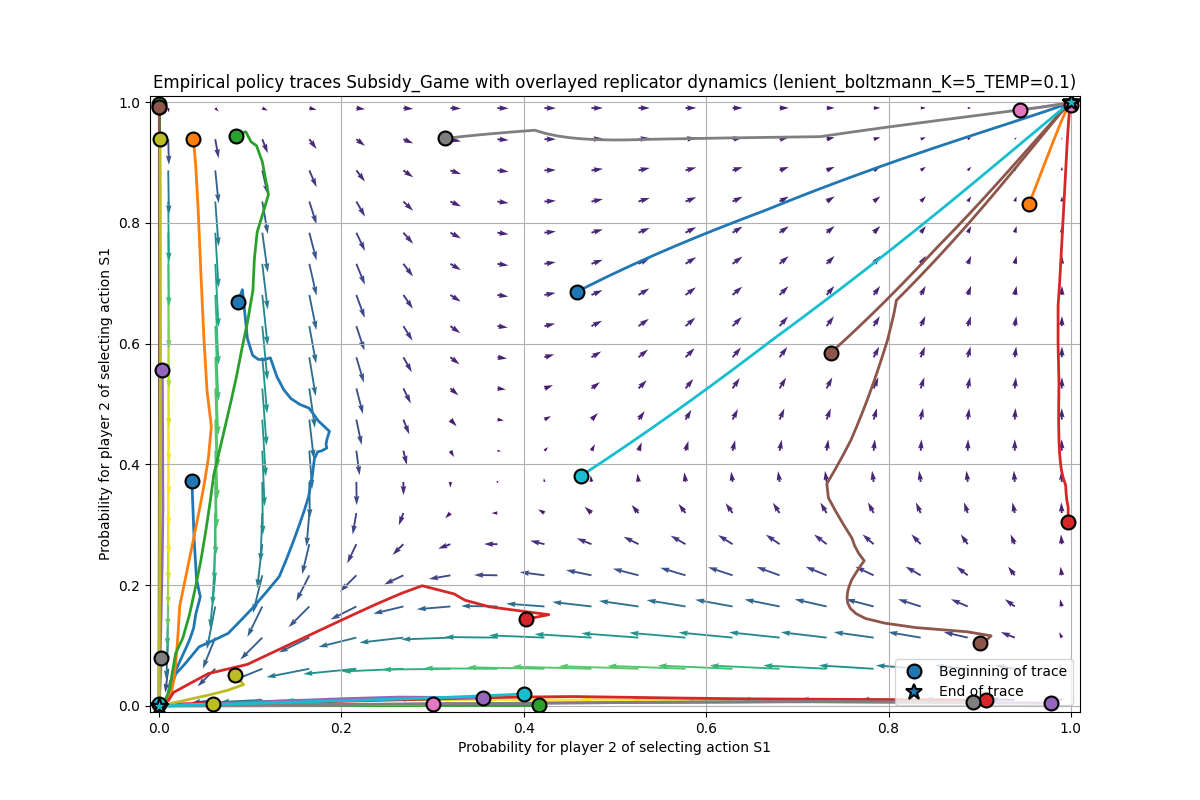
\includegraphics[width=\linewidth]{plots/replicator_trajectoreis_Subsidy_Game_lenient_boltzmann_K=5_TEMP=0.1.png}
        \caption{Subsidy Game}
        \label{fig:lbsg}
    \end{subfigure}
    \hfill
    \begin{subfigure}{0.49\textwidth}
        \centering
        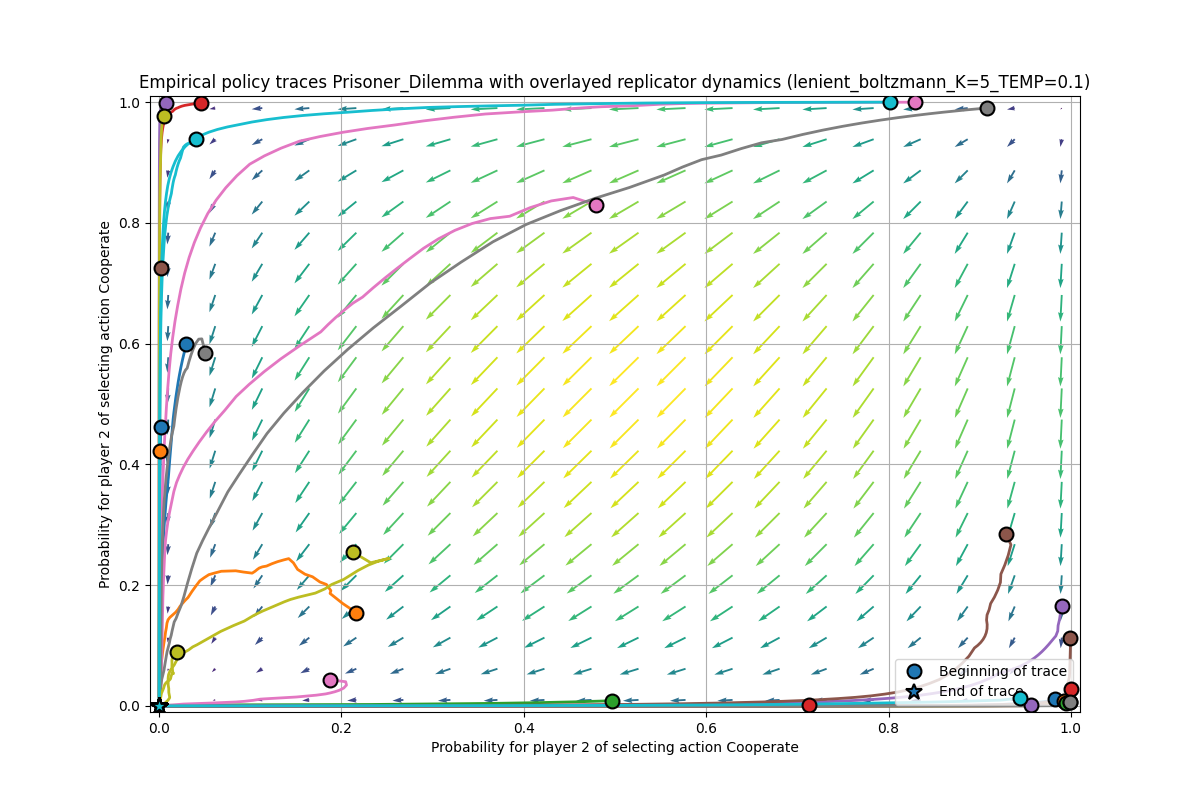
\includegraphics[width=\linewidth]{plots/replicator_trajectoreis_Prisoner_Dilemma_lenient_boltzmann_K=5_TEMP=0.1.png}
        \caption{Prisoner's Dilemma}
        \label{fig:lbpd}
    \end{subfigure}
    \caption{Empirical policy traces for Lenient Boltzmann Q-Learning (K=5, temperature = 0.1), (a) Subsidy Game and (b) Prisoner's Dilemma.}
    \label{fig:lenient_combined}
\end{figure}
\paragraph{Convergence Analysis (temperature=0.1, K=5, lr=0.1)}
We analyzed the convergence of Lenient Boltzmann Q-Learning regarding Nash Equilibria (NE) and Pareto Optimality (PO):

\begin{itemize}
    \item \textit{Stag Hunt:} Almost all traces converged to the (Stag, Stag) Nash Equilibrium (NE),
          which is also Pareto Optimal (PO). A few converged to the (Hare, Hare) NE.
    \item \textit{Subsidy Game:} Traces split roughly evenly between the two NEs: (Subsidy 1, Subsidy 1) (which is PO)
          and (Subsidy 2, Subsidy 2) (which is not PO), with slight preference for (Subsidy 2, Subsidy 2).
    \item \textit{Matching Pennies:} Traces did not converge (random strategy), consistent with the lack of a pure strategy NE.
          All outcomes in this game are PO.
    \item \textit{Prisoner's Dilemma:} All traces converged to the (Defect, Defect) NE, which is not PO, no matter the initialization.
\end{itemize}

Convergence to an existing NE occurred in all applicable games. A strong preference for converging to a
single equilibrium was observed, often regardless of initialization. Based on our experiments, this tendency
strengthened with higher K values (e.g., K=25).

\paragraph{How K affects the results}

Higher K values lead to a stronger preference to converge to a Nash Equilibrium solution, even if the solution is far from the starting point.
For $K=25$, the initialization almost does not matter, the algorithm will almost always converge to the same solution.

Interestingly, for the Subsidy Game (Fig. \ref{fig:combined_subsidy}), depending on the $K$ value, the algorithm will converge to different Nash Equilibria.
For $K=2$ the algorithm converged to (Subsidy 1, Subsidy 1) and for $K=25$ it converged to (Subsidy 2, Subsidy 2). This shows that the algorithm
explores better when the $K$ value is higher and finds better solutions. However, as explained in section \ref{sec:lenient},
the algorithm will always prefer a Nash Equilibrium solution over a Pareto Optimal solution, as it does not rely on the opponent's goodwill.
This is displayed clearly by the Prisoner's Dilemma, where the algorithm always converged to (Defect, Defect), completely ignoring
the Pareto Optimal solution (Cooperate, Cooperate).

\begin{figure}[h]
    \centering
    \begin{subfigure}{0.49\textwidth}
        \centering
        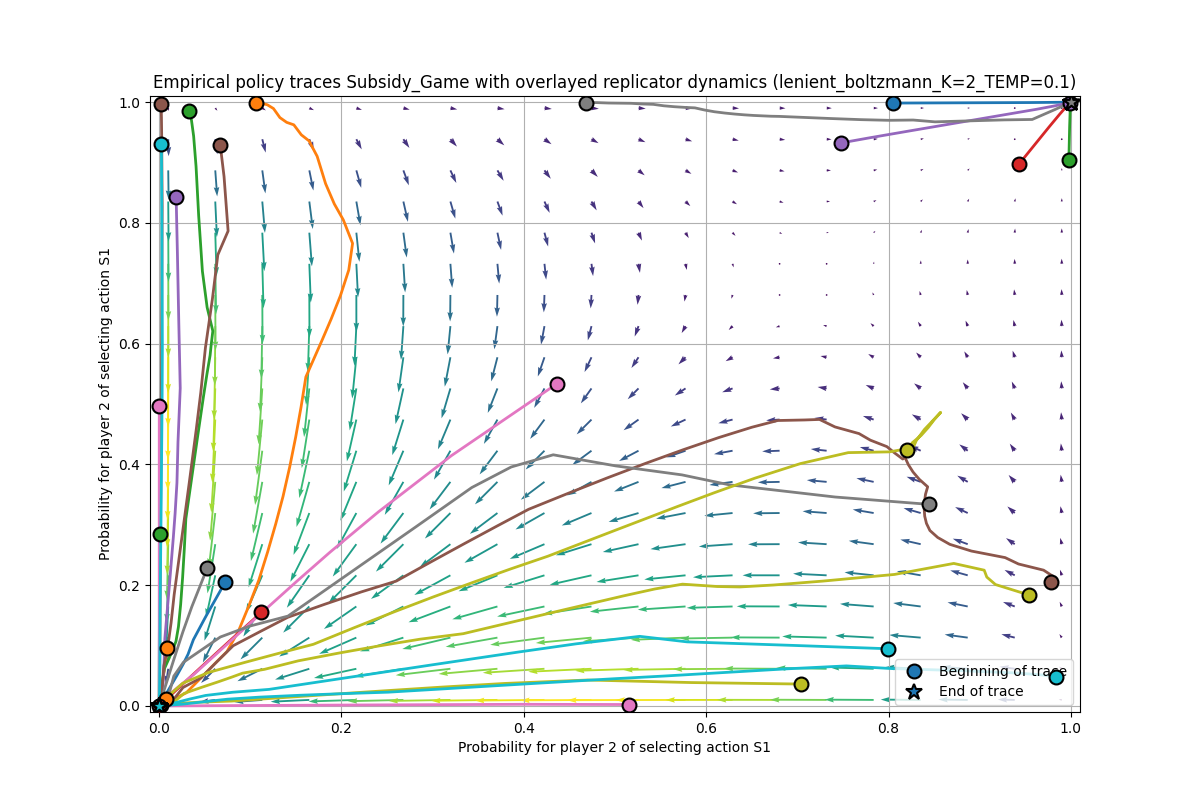
\includegraphics[width=\linewidth]{plots/replicator_trajectoreis_Subsidy_Game_lenient_boltzmann_K=2_TEMP=0.1.png}
        \caption{K=2, temperature = 0.1}
        \label{fig:sfiglbshk1}
    \end{subfigure}
    \hfill
    \begin{subfigure}{0.49\textwidth}
        \centering
        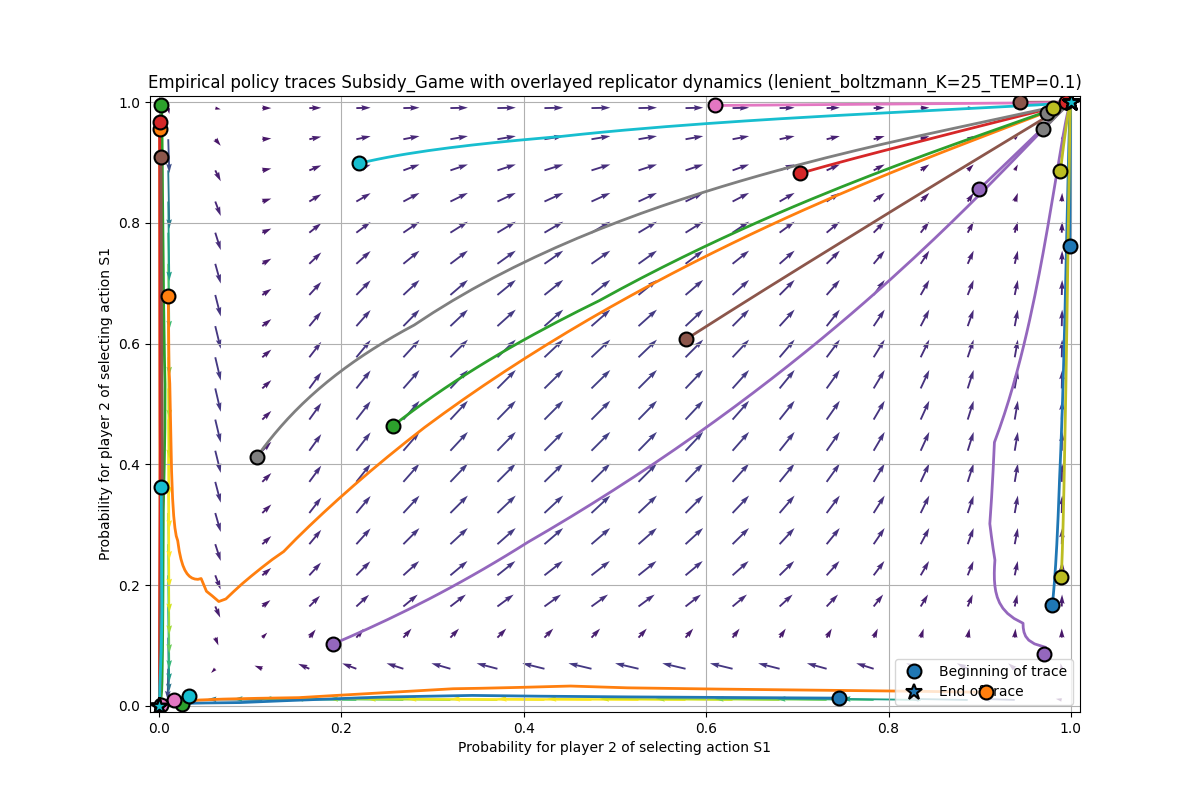
\includegraphics[width=\linewidth]{plots/replicator_trajectoreis_Subsidy_Game_lenient_boltzmann_K=25_TEMP=0.1.png}
        \caption{K=25, temperature = 0.1}
        \label{fig:sfiglbshk2}
    \end{subfigure}
    \caption{Empirical policy traces for Lenient Boltzmann Q-Learning on the Subsidy Game showing the effect of different K values: (a) K=2 shows more dependence on initial conditions, while (b) K=25 demonstrates stronger convergence to a single solution regardless of starting points.}
    \label{fig:combined_subsidy}
\end{figure}

\subsection{Replicator Dynamics}

% DONE: dimitris check if you like this line taht learnign traces does nto alwsy follow replicator dynamics
% Yes I love the line, it's very interesting.
The Empirical policy traces are behaving as expected and follow the replicator dynamics, as the replicator dynamics are a set of differential equations
that describe the evolution of the population of strategies in a game, so individual strategies are going to naturally follow their path.

Some exceptions exist to this rule, like the Prisoner's Dilemma, when using the Boltzmann Q-Learning algorithm, where the algorithm
does not follow the replicator dynamics. The cause of this is the probabilistic nature of the algorithm.
In cases where both players decide to cooperate, the algorithm will prefer the Pareto Optimal solution (Cooperate, Cooperate)
over the Nash Equilibrium (Defect, Defect), as it gives a better reward. This is not the case for the Lenient Boltzmann Q-Learning algorithm,
where the algorithm will explore multiple potential actions and thus is more likely to Defect as a response to the opponent's action.
In simple terms, Boltzmann Q-Learning is more likely to trust the opponent and thus is more likely to cooperate, because it only explores one action.

\section{\textbf{Task 3:}}

For task 3, we need to train an agent to play the game Knights Archers Zombies (KAZ), which is a Butterfly environment from PettingZoo \cite{pettingzoo}.
In this implementation, we are asked to have only archers as agents, making the game more complex as the agents need to calculate
angles, distances, and predict the movement of the zombies. This provides enough of a challenge for simple agents to learn the game and be able to play it well.

\subsection{Baseline Agent}
We have implemented two baseline agents. First, a random agent, which picks actions randomly. Second, a diagonal agent, which goes to the bottom right corner
and shoots straight to the left, parallel to the bottom edge.

\subsection{Research Questions}
Several reinforcement learning algorithms are trained to play in environments like PettingZoo. One of the more commonly used ones is PPO \cite{albrecht},
which was also proposed in the project description. On the other hand, several other algorithms were state-of-the-art in these environments,
like IMPALA \cite{impala}, when first developed. So, we decided to implement both of them and compare their performance to see
if PPO can compete with IMPALA in this environment. Which model can learn and play Knights Archers Zombies (KAZ) better?

\subsection{Algorithms}
The first algorithm implemented is \textbf{Proximal Policy Optimization (PPO)} \cite{schulman2017}.
PPO ensures stable policy improvements using a clipped surrogate objective function that constrains update magnitudes,
preventing large policy changes.
It employs an actor-critic architecture where advantage estimation determines the relative value of actions.
This approach balances learning efficiency with implementation simplicity, making PPO widely adopted for complex reinforcement learning tasks.

The second algorithm implemented is the \textbf{Importance Weighted Actor-Learner Architecture (IMPALA)} \cite{impala}.
This algorithm has an off-policy actor-critic architecture designed to be easily parallelized and distributable. Actors are responsible for
generating trajectories in the environment using a policy $\mu$ and sending them to the learner, which is responsible for updating its policy $\pi$.
The main innovation of this algorithm is the use of a V-trace, which is a method of correcting the lag between the actor and the learner policies.
The algorithm was originally tested in environments similar to PettingZoo (i.e., DMLab-30 and Atari-57 \cite{impala}), giving impressive results.

From the results that already exist in the literature, and since IMPALA was designed specifically to handle arcade environments,
we can expect that IMPALA will outperform PPO in KAZ.

\subsection{Feature Engineering}

The library provided by PettingZoo provides 2 ways of getting the state of the game. The default way is to use a vector that contains
information about the position of the agents and the zombies, as well as the distance between them and directional vectors.
This is a very simple way of getting the state of the game, but it still provides a lot of information for the agent to learn from.
This is the main representation used in the implementation of the PPO and IMPALA algorithms.

The vector was manually modified to include the three extra components to help the agent evaluate a zombie's threat level. Specifically, the three extra components are:
Zombie distance to bottom edge, Zombie deviation from screen center, and Zombie urgency (bottom distance with higher value for closer zombies).

These metrics are used to give more information to the agent about the state of the game and help it learn faster. %...results?...

Another improvement is the removal of the rows about the arrows from the vector. The arrows are not immediately relevant to the agent as they have very predictable behavior so they don't add a lot of value
to the representation. Removing them removes a lot of noise and allows for the agent to focus on the position of the zombies.

% DONE: is this correct/ do pixels give more info?
% Arrow direction, pixel detail, and the fact that it's the same data a human would see, it's more accurate, but not better. Vector is more efficient.
The second way is to use a pixel representation of the game, which is a more accurate way of getting the state of the game. This representation provides a lot more information for the agent to learn from,
but it also contains a lot of irrelevant data (specifically empty spaces). This method also required a lot more computational resources to train the agent and was more difficult to train.

\subsection{Implementation \& Training}

For \textbf{PPO}, we started experimenting with hyperparameters manually and decided on them through a trial-and-error approach.
Once we had a set of hyperparameters that worked well enough, we chose a few to fine-tune with a grid search approach.
The parameters we chose to fine-tune were rollout fragment length, whether or not to use KL loss, the maximum number of cycles for a game, and whether or not to use arrows as a feature.
During the exploration phase of the algorithms, we have noticed that they have a significant effect on the results.

The exact configuration of the grid search space can be found in the appendix.
The final set of hyperparameters is shown in Table \ref{tab:hyperparameters}.

% DONE: add proper params for IMPALA
\begin{table}[h]
    \centering
    \begin{tabular}{|l|l|l|}
        \hline
        \textbf{Parameter}           & \textbf{PPO}                  & \textbf{IMPALA}          \\
        \hline
        Network architecture         & FCNET [256, 128], ReL         & FCNET [256, 128], ReLU   \\
        \hline
        VF share layers              & False                         & True                     \\
        Use LSTM                     & -                             & False                    \\
        \hline
        Rollout fragment length      & 512                           & 512                      \\
        Train batch size             & 4096 = (512 $\cdot$ 8)        & 4096 = (512 $\cdot$ 8)   \\
        \hline
        Learning rate                & [0, 3e-4],[1.5M, 1e-4]        & [[0, 1e-3], [10M, 1e-4], \\
                                     & [3M, 5e-5], [4M, 1e-5]        & [20M, 1e-5]]             \\
        \hline
        Entropy coefficient          & [[0, 0.015],  [1M, 0.010]     & 0.01                     \\
                                     & [2.5M, 0.005], [3.5M, 0.002]] &                          \\
        \hline
        Discount factor              & 0.99                          & 0.99                     \\
        Value function coeff         & 0.5                           & 0.5                      \\
        Gradient clip                & 0.5                           & 1.0                      \\
        SGD iterations               & 10                            & 10                       \\
        \hline
        GAE lambda                   & 0.95                          & -                        \\
        PPO clip param               & 0.2                           & -                        \\
        Value function clip          & 10.0                          & -                        \\
        KL loss, coefficient, target & True, 0.2, 0.01               & -                        \\
        \hline
        vtrace                       & -                             & True                     \\
        \hline
        Use arrows features          & False                         & False                    \\
        Max cycles                   & 1000000                       & 1000000                  \\
        \hline
    \end{tabular}
    \caption{Hyperparameters for single-agent PPO and IMPALA}
    \label{tab:hyperparameters}
\end{table}


Initially, we hypothesized that a longer rollout length, as well as using arrows as features, would produce better results.
We expected that using KL loss would make training more stable, but would not necessarily result in a better policy.

We were unsure whether longer maximum cycles would be better, as they are not a direct parameter of the algorithm and only allow the agent player more time.
However, it does not need to lead to a better policy in the end.

Due to limited computational resources, we trained only 16 configurations for 1000 epochs each.

We found that the best model uses 1000000 max cycles, a rollout length of 512, uses KL loss, but does not use the arrow features.

It is clear that the most crucial parameter is rollout length.
There is not a single model using 256 rollout length that would perform better than any of the models using 512.
Using KL loss seems to help. In particular, when you look at the learning trajectories,
they are significantly smoother and without dips. This is expected because KL loss penalizes large changes in the policy.
On average, using max cycles of 2000 produces better results, though the best model uses 10000000.

Interestingly, the best model does not use arrows as features and produces significantly better
results than any other model. This could be just a lucky coincidence, as this is one of the few
models that had a learning trajectory (Fig. \ref{fig:learning_trajectory_best_single}) without any major dips, which was very uncommon for most configurations.

To \textbf{evaluate} and \textbf{select} the best configuration, we could not rely on average return, as varying the maximum number of cycles directly affects the final reward—the more cycles,
the higher the possible reward. Low maximum cycles can terminate the agent before it fails, but this does not necessarily reflect policy quality.
Therefore, we chose the second-best configuration by average reward and the second-to-last by epochs. Each was evaluated with 50 seeds for
both 10,000 and 10,000,000 maximum cycles, and the best was selected based on these results, with preference to look at the results of the 10,000,000 maximum cycles.

We sampled actions from the model rather
than using a greedy policy, as sampling empirically yielded better outcomes. We avoided the best and last models because performance
plateaued after the best, suggesting no further policy improvement; thus, the second-best was likely more robust. With more time and
resources, we would have further validated this approach and explored better model checkpoint selection.

\textbf{IMPALA} was trained differently, as it is a more complex algorithm and requires a different approach to training.
The values for the hyperparameters were transferred from the PPO implementation, so that there is a fair comparison between the two algorithms.
This provided a good starting point for the training of the IMPALA algorithm. But it was immediately apparent that the algorithm was not learning fast enough.
This was quickly attributed to the learning rate, which was set too low. The learning rate was increased to 0.001, and the algorithm started to learn much faster.

Other parameters that are important to mention are the use of V-trace, which is a method of correcting the lag between the actor and the learner policies.
This is a very important part of the algorithm and is one of the main reasons why IMPALA can perform so well.

In one of the experiments, we also tried to use the pixel representation of the game. This method was inspired by the work of \cite{impala},
where they used a pixel representation of the game to train their agents. This was outperformed by the vector representation of the game.
The vector representation provided a much smaller state space and was much easier to train.
The pixel representation was also much more difficult to train because it required a lot more computational resources.

Another aspect of IMPALA that was dropped was the use of LSTM. This was done because they provided minimal improvement in the results, and
at the cost of a lot of training time. The environment has very little temporal correlation, so little use for long-term memory, so the use of LSTM was not necessary.

Finally, the entropy coefficient was set to 0.01, which helps the agent to explore the state space and avoid premature convergence.
This, although good for the earlier stages of training, is the main suspect for the high variance in the results in the later stages of training.
This is seen in the learning trajectory of IMPALA (Fig. \ref{fig:learning_trajectory_best_single}).

\paragraph{Results}

To evaluate the performance of the agents, we used the average return per agent along with the standard deviation, across 50 different seeds and 10000000 max cycles.

Random agent got score  1.96, while the diagonal agent got 36.2, which is surprisingly good.

\begin{table}[h]
    \centering
    \begin{tabular}{|l|l|l|}
        \hline
        \textbf{Agent}          & \textbf{Average Return} & \textbf{Standard Deviation} \\
        \hline
        Random agent            & 1.96                    & 1.84                        \\
        Diagonal agent          & 36.2                    & 31.21                       \\
        \hline
        PPO single agent        & 467.68                  & 468.89                      \\
        IMPALA single agent     & 408.6                   & 318.39                      \\
        \hline
        PPO multi agent         & 126.85                  & 83.95                       \\
        IMPALA multi agent      & 172.32                  & 194.23                      \\
        \hline
        PPO tournament          & 106.5                   & -                           \\
        IMPALA tournament       & 107.46                  & -                           \\
        \hline
        PPO tournament multi    & 74.75                   & -                           \\
        IMPALA tournament multi & 54.2                    & -                           \\
        \hline
    \end{tabular}
    \caption{Evaluation results for PPO and IMPALA on 50 seeds and 10000000 max cycles.}
    \label{tab:results}
\end{table}

The first comment that needs to be made about the results is that the agents massively outperform the baselines. This means that they learn to play
the game and don't just adopt a simple tactic.

Going further than that, for the single agent, both models seem to give similar results. That is, they produce very high averages (in the 400s) without issue and
can score 100+ in the tournaments. % DONE: Jan fact check this  (JAN: i kind of changed it to 100+ to be more general and left out 'consistently')
A better comparison in this case is the standard deviation because it can indicate the likelihood that a model gets some very bad games that could
result in a bad score. IMPALA, in this case, has a lower standard deviation, so it is considered more appropriate for the tournament.

The results are some what surprising. It was expect that IMPALA would significantly outperform the competition, as it's supposedly one of the better algorithms
for arcade game like environments. PPO preforms masterfully in this environment, giving high quality results. Significant portion of this can be attributed
to the state vector as it simplifies the environment to a level much more manageable to the algorithms and thorough fine-tuning of the hyperparameters.

For the full table with evaluation data of PPO, please see Table \ref{tab:multi_ppo_results} in the Appendix.

\paragraph{Agent Behavior PPO}
Agent learned to keep to the bottom line and to the left corner most of the time. They start to shoot down zombies from there by firing volleys of arrows at zombies.
What one may find surprising is that the agent is not particularly good at predicting the movement of the zombies and shooting accordingly.
We have noticed that agent have particular problems with shooting down zombies that are very close to the bottom line.
Overall, the agent is rather static and does not move much, besides rotating in the direction of the zombies.

\begin{figure}[h]
    \centering
    \begin{subfigure}[b]{0.48\textwidth}
        \centering
        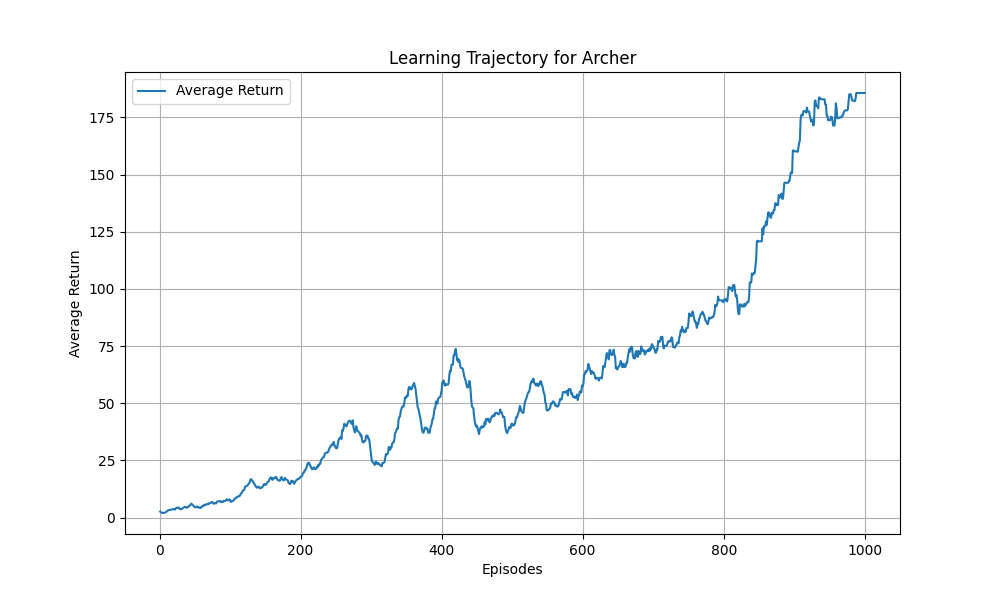
\includegraphics[width=\linewidth]{figures_latex/learning_trajectory_ppo_best.png}
        \caption{PPO}
        \label{fig:learning_trajectory_ppo_best}
    \end{subfigure}
    \hfill
    \begin{subfigure}[b]{0.48\textwidth}
        \centering
        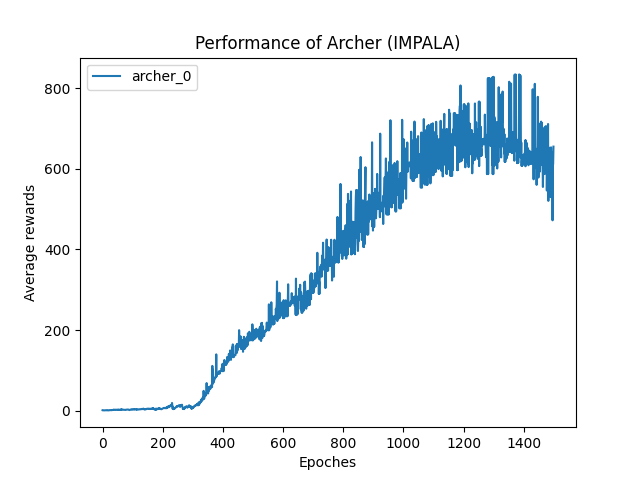
\includegraphics[width=\linewidth]{figures_latex/lt_single_impala_best.png}
        \caption{IMPALA}
        \label{fig:learning_trajectory_impala_best}
    \end{subfigure}
    \caption{Learning trajectories of the best models for single agent for (a) PPO over 1000 epochs and (b) IMPALA over 1500 epochs}
    \label{fig:learning_trajectory_best_single}
\end{figure}

\paragraph{Agent Behavior IMPALA}
The IMPALA agent learns to move around the map quite comfortably and has no trouble dealing with zombies in any part of the board.
The agent displayed all the behaviors of a good player, having no problems with sniping zombies from across the map, and managing his distance from the zombies easily.
He has also been observed shooting a wall of arrows horizontally or diagonally to catch zombies that are going to pass by his position.
Targeting zombies that have passed his position (i.e., that are closer to the wall than him) has also been observed, which is a very good behavior.
Stressful situations (i.e., when zombies are close to the bottom line and there are also zombies near him) are handled well, as the agent is able to shoot and move,
managing both threats at the same time.

Finally, the agent has been seen "quitting" the game by moving erratically. This is concerning as it's unclear as to why he does that. % at some point he has spinning around himself.
The theory is that this happens when he predicts that he is going to lose, which would be a reasonable behavior.

\section{\textbf{Task 4: Playing Multi-Agent Knights-Archers-Zombies}}

\subsection{Implementation \& Evaluation}

We used the same algorithms and hyperparameters as in the single-agent case. The only changes we made were
to the network architecture, setting it to FCNET$[512,256,128]$, and the reward schema,
so that no matter which agent kills the zombie, both agents are rewarded.
We have trained agents without and with a modified reward schema, and experiments show that using the modified
reward schema produces significantly better results.

Learning trajectories for the multi-agent case are shown in Fig. \ref{fig:multi_agent_learning_curves}.

The most significant adaptation for the multi-agent case was to use a shared policy for both agents.
The reason for this is that both agents are the same and have the same purpose, action space, and observation
space, making it more efficient to train a single policy for both agents. We did not implement any explicit
communication between agents, as we believed that having implicit communication in the form of full knowledge
of the state of the game would be enough to achieve good results.

We have evaluated and chosen the best model checkpoint in the same manner as for the single-agent case.
See Table \ref{tab:results} for full evaluation results of the multi-agent case.

When it comes to the question of which of the two models is better, the opposite of the single agent is true. While IMPALA gets some high averages,
it also has very high deviation. I this case PPO, is considered better as it gives more consistent results, as can be seen in the tournament results \ref{tab:results}.
The agents seem to perform worse compared to single agents. This happens probably due to poor communication, as they often target the zombies.
One other problem observed is the lack of concern for the archer's life, as the game will still be played by the other player, and
the dead archer will still get rewards for the other archer's kills.

\subsection{Discussion and observations}

For \textbf{PPO}, agents consistently group on the map's left side, preferring the top line, which often results in
death from nearby zombie spawns. Their strategy involves simultaneous arrow volleys in the same direction.
No specialization was observed; agents typically attack the same zombie concurrently, a potentially suboptimal tactic.
Occasionally, if a nearby zombie approaches, one agent retreats while the other shoots. While adept at predicting
zombie movement, they seem not to trust their observations, firing continuously until the zombie is dead, wasting
time. As in the single-agent case, agents struggle with zombies near the bottom line, often ignoring them to
target less immediate threats. This surprising behavior might be due to the infrequency of such situations,
which usually lead to a fast defeat.

For \textbf{IMPALA}, agents behave similarly to PPO. They are not coordinated and often attack the same zombie.
This is the most concerning behavior, as it is a waste of arrows and time. It clearly shows a lack of quality communication.
They also tend to be less concerned about zombies that are close to them, often leading to their death.
Probably because of a lack of penalization for agent death in the reward schema.
They tend to move fine around the map and target zombies close and far from them, but that is the extent of good behavior.

\paragraph{Future Directions}
Several avenues could be could be explored to improve the performance of the multi-agent case:

\textbf{Centralized Policy:} Explore the use of a centralized training with decentralized execution (CTDE) approach.
This could enable better coordination and possibly allow for specialization between agents.

\textbf{Explicit Communication:} Implement explicit communication mechanisms between agents. This may help agents share information
about the environment or their intentions, leading to more sophisticated strategies.

\textbf{Arrows usage:} Reconsider the removal of arrows from the observation vector. While this was beneficial in the single-agent setting,
arrows may provide valuable information about actions of other agents in the multi-agent case.

\textbf{Reward Shaping:} Investigate the effects of penalizing the death of individual agents.
This could encourage agents to act more cautiously and improve overall survival.

\textbf{Checkpoint Selection:} Systematically evaluate more model checkpoints to ensure the best-performing policy is selected.

\begin{figure}[H]
    \centering
    \begin{subfigure}[b]{0.49\textwidth}
        \centering
        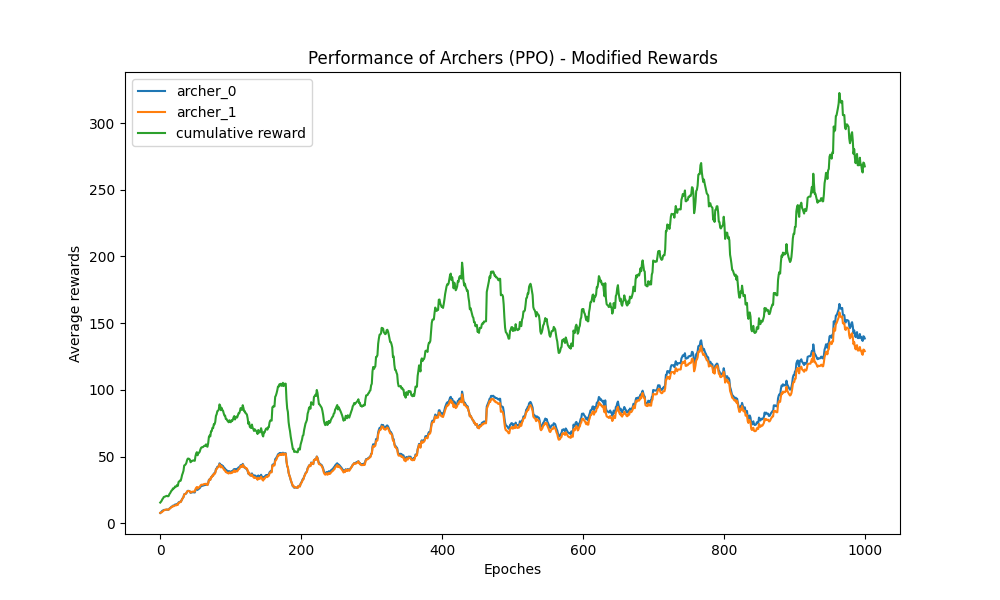
\includegraphics[width=\linewidth]{figures_latex/learning_trajectory_multi_ppo.png}
        \caption{Learning curve for multi-agent PPO of combined reward for both agents over 1000 epochs using modified rewards schema.}
        \label{fig:sfiglbshk25}
    \end{subfigure}
    \hfill
    \begin{subfigure}[b]{0.49\textwidth}
        \centering
        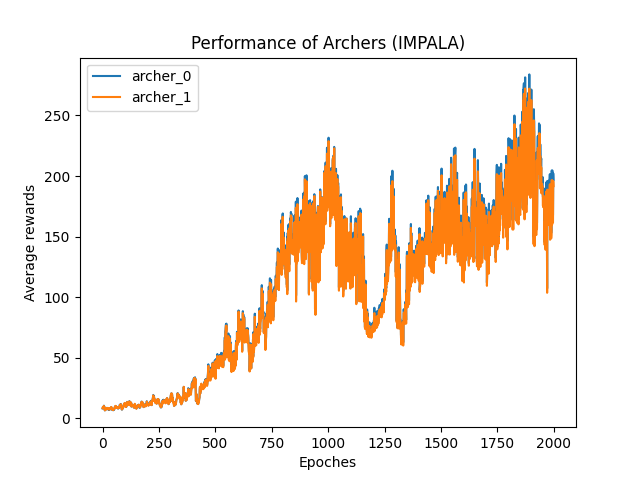
\includegraphics[width=\linewidth]{figures_latex/lt_multi_impala_best_mod_rewards.png}
        \caption{Learning curve for multi-agent IMPALA of combined reward for both agents over 2000 epochs using modified rewards schema.}
        \label{fig:sfiglbshk26}
    \end{subfigure}
    \caption{Learning curves for multi-agent (a) PPO and (b) IMPALA using modified rewards schema.}
    \label{fig:multi_agent_learning_curves}
\end{figure}



\begin{thebibliography}{9}
    \bibitem{shoham}
    Yoav Shoham and Kevin Leyton-Brown. Multiagent Systems: Algorithmic, Game-Theoretic, and Logical Foundations. Cambridge University Press, 2009. URL: http://www.masfoundations.org/mas.pdf.

    \bibitem{busoniu}
    L. Buşoniu, R. Babuška, and B. De Schutter, "A comprehensive survey of multi-agent reinforcement learning," IEEE Transactions on Systems, Man, and Cybernetics, Part C: Applications and Reviews, vol. 38, no. 2, pp. 156-172, Mar. 2008. doi:10.1109/TSMCC.2007.913919

    \bibitem{bloembergen}
    Bloembergen, D., Tuyls, K., Hennes, D., \& Kaisers, M. (2015). Evolutionary Dynamics of Multi-Agent Learning: A Survey. In Journal of Artificial Intelligence Research (Vol. 53, pp. 659-697). AI Access Foundation. https://doi.org/10.1613/jair.4818

    \bibitem{pettingzoo}
    Terry, J. K., Black, B., Grammel, N., Jayakumar, M., Hari, A., Sullivan, R., Santos, L., Perez, R., Horsch, C., Dieffendahl, C., Williams, N. L., Lokesh, Y., \& Ravi, P. (2020). PettingZoo: Gym for Multi-Agent Reinforcement Learning (Version 7). arXiv. https://doi.org/10.48550/ARXIV.2009.14471

    \bibitem{albrecht}
    Stefano V. Albrecht, Filippos Christianos, and Lukas Schäfer. Multi-Agent Reinforcement Learning: Foundations and Modern Approaches. MIT Press, 2024.

    \bibitem{schulman2017}
    Schulman, J., Wolski, F., Dhariwal, P., Radford, A., \& Klimov, O. (2017). Proximal Policy Optimization Algorithms. arXiv:1707.06347.

    \bibitem{impala}
    Espeholt, L., Soyer, H., Munos, R., Simonyan, K., Mnih, V., Ward, T., Doron, Y., Firoiu, V., Harley, T., Dunning, I., Legg, S., \& Kavukcuoglu, K. (2018). IMPALA: Scalable Distributed Deep-RL with Importance Weighted Actor-Learner Architectures (Version 3). arXiv. https://doi.org/10.48550/ARXIV.1802.01561

\end{thebibliography}


\newpage

\begin{appendices}
    \section{Learning trajectories and replicator dynamics}

    \subsection{$\epsilon$-Greedy Q-Learning}

    \begin{figure}[H]
        \centering
        \begin{subfigure}{0.44\textwidth}
            \centering
            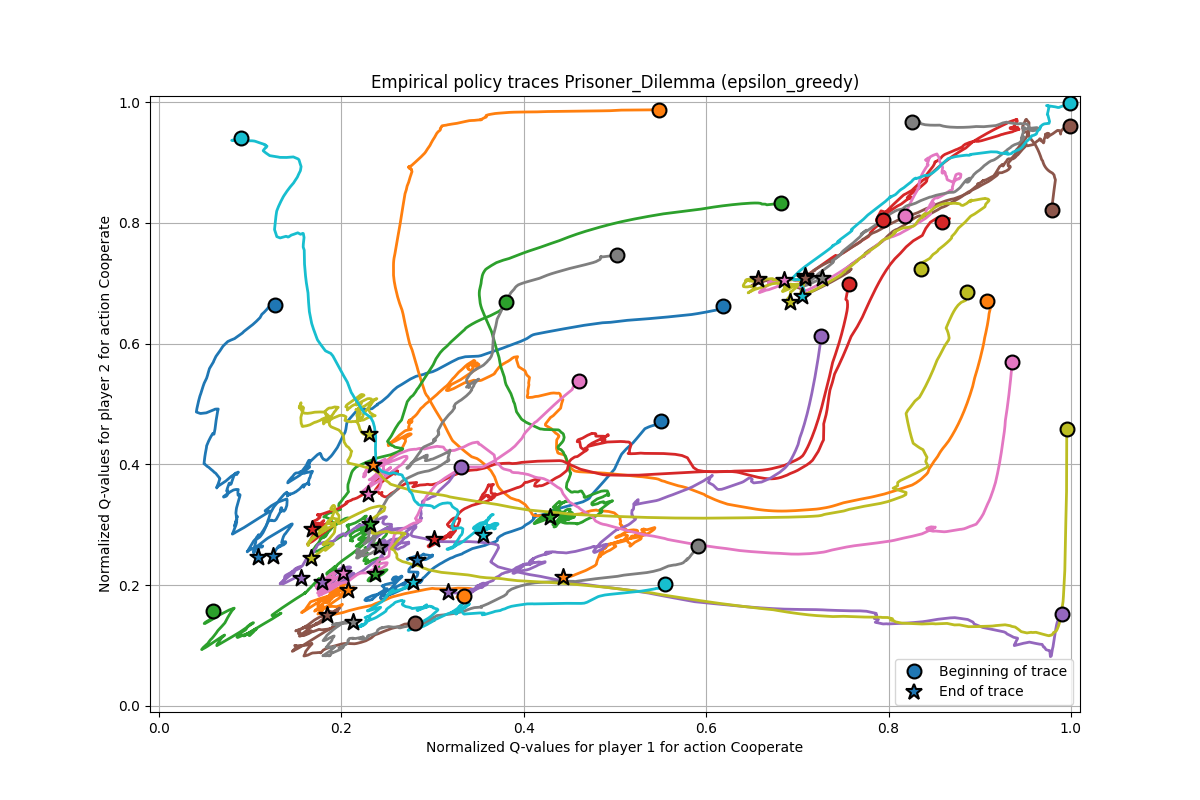
\includegraphics[width=\linewidth]{plots/replicator_trajectoreis_Prisoner_Dilemma_epsilon_greedy.png}
            \caption{Prisoner's Dilemma}
        \end{subfigure}
        \hfill
        \begin{subfigure}{0.44\textwidth}
            \centering
            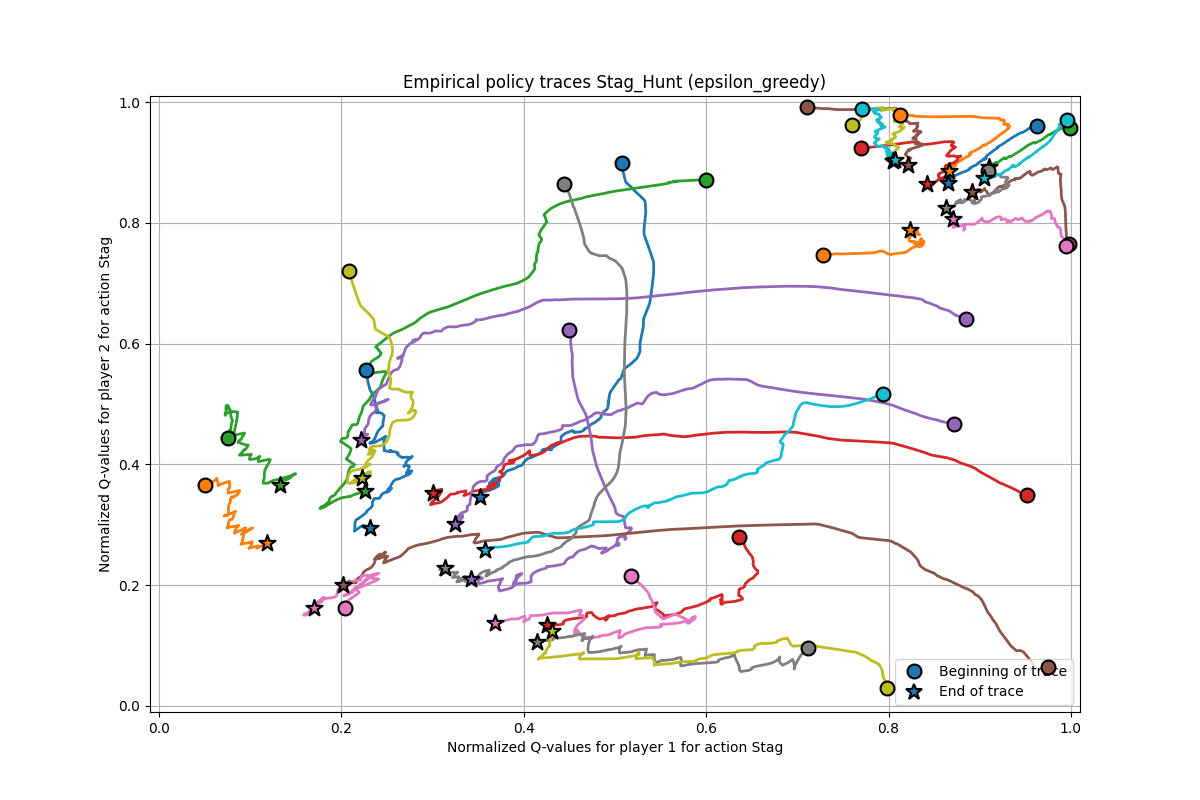
\includegraphics[width=\linewidth]{plots/replicator_trajectoreis_Stag_Hunt_epsilon_greedy.png}
            \caption{Stag Hunt}
        \end{subfigure}
        \vspace{0.5cm}
        \begin{subfigure}{0.44\textwidth}
            \centering
            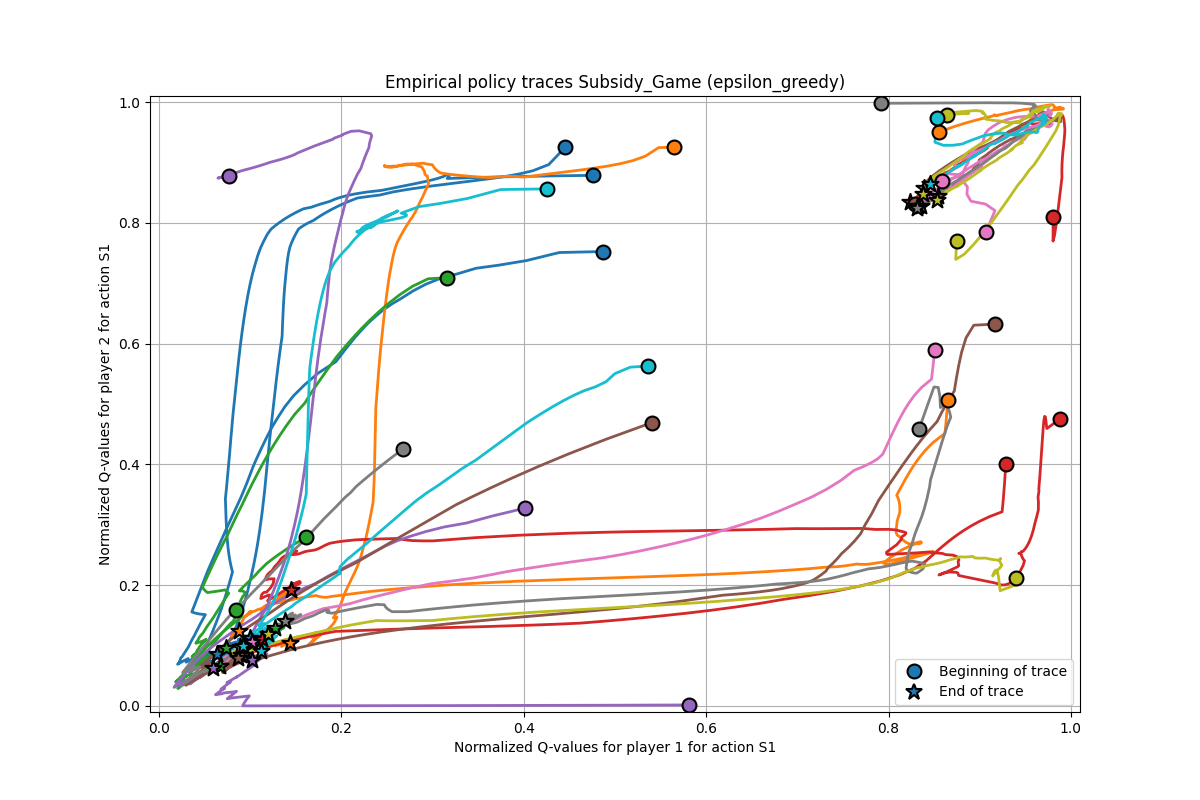
\includegraphics[width=\linewidth]{plots/replicator_trajectoreis_Subsidy_Game_epsilon_greedy.png}
            \caption{Subsidy Game}
        \end{subfigure}
        \hfill
        \begin{subfigure}{0.44\textwidth}
            \centering
            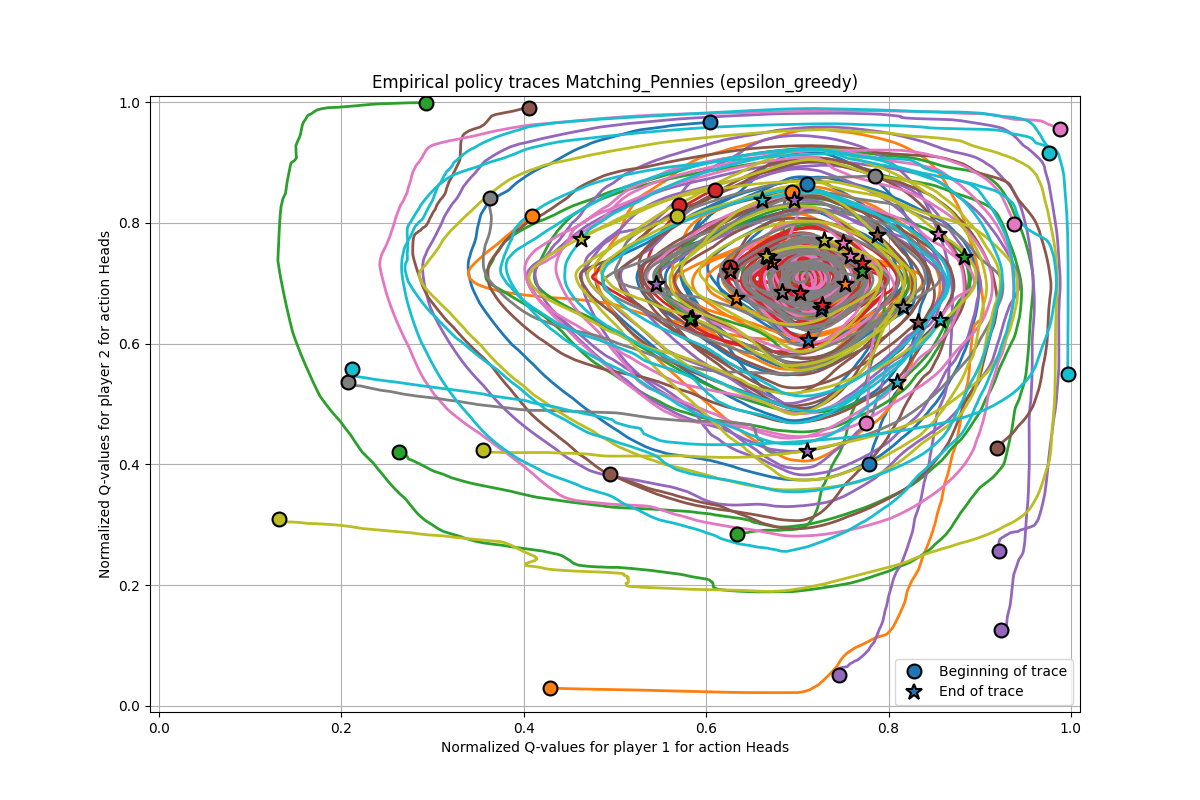
\includegraphics[width=\linewidth]{plots/replicator_trajectoreis_Matching_Pennies_epsilon_greedy.png}
            \caption{Matching Pennies}
        \end{subfigure}
        \caption{Empirical policy traces for $\epsilon$-Greedy Q-Learning ($\epsilon=0.1$) across different games.}
        \label{fig:app_epsilon_greedy_combined}
    \end{figure}

    \subsection{Boltzmann Q-Learning}

    \begin{figure}[H]
        \centering
        \begin{subfigure}{0.44\textwidth}
            \centering
            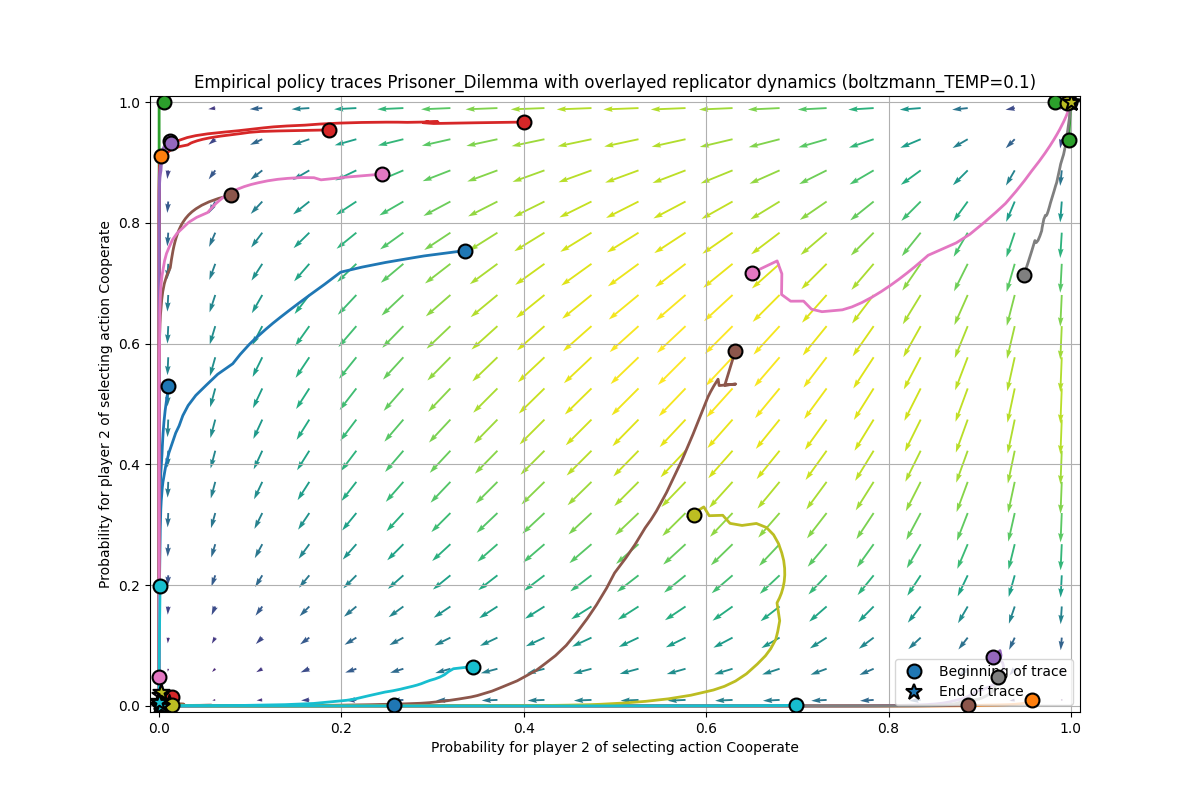
\includegraphics[width=\linewidth]{plots/replicator_trajectoreis_Prisoner_Dilemma_boltzmann_TEMP=0.1.png}
            \caption{Prisoner's Dilemma}
        \end{subfigure}
        \hfill
        \begin{subfigure}{0.44\textwidth}
            \centering
            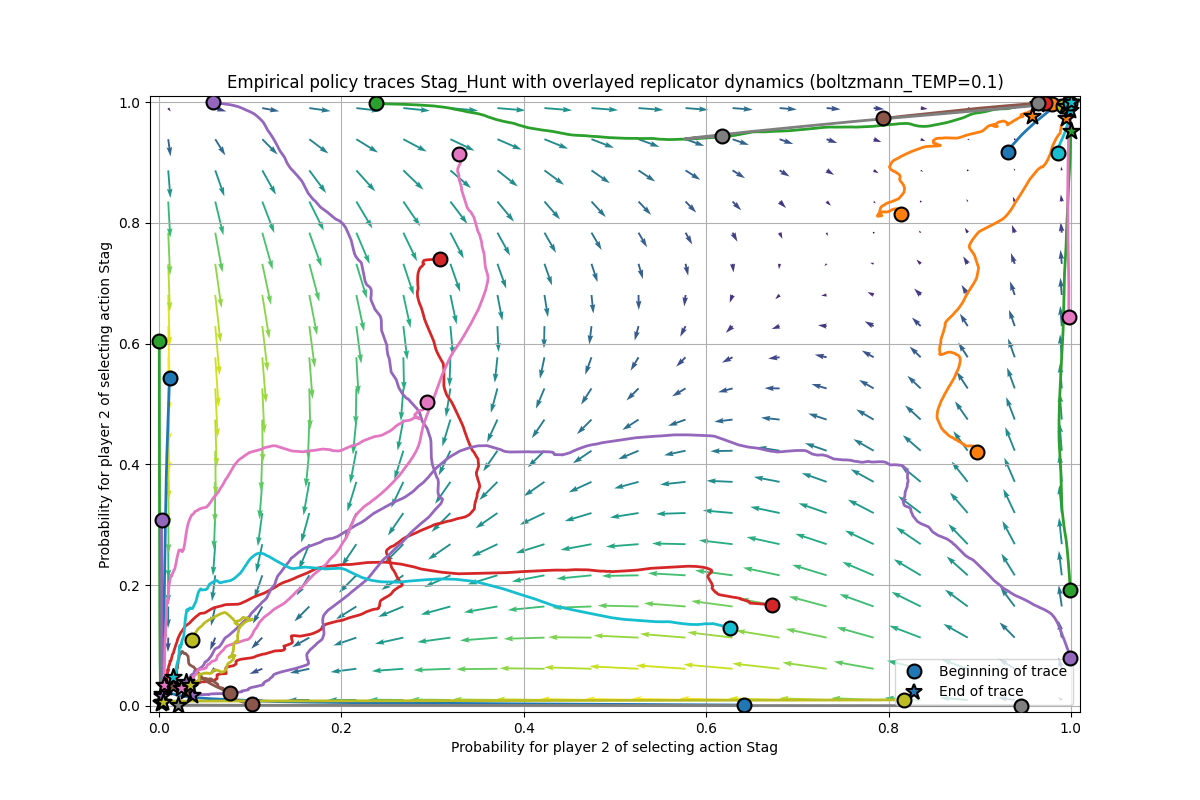
\includegraphics[width=\linewidth]{plots/replicator_trajectoreis_Stag_Hunt_boltzmann_TEMP=0.1.png}
            \caption{Stag Hunt}
        \end{subfigure}
        \vspace{0.5cm}
        \begin{subfigure}{0.44\textwidth}
            \centering
            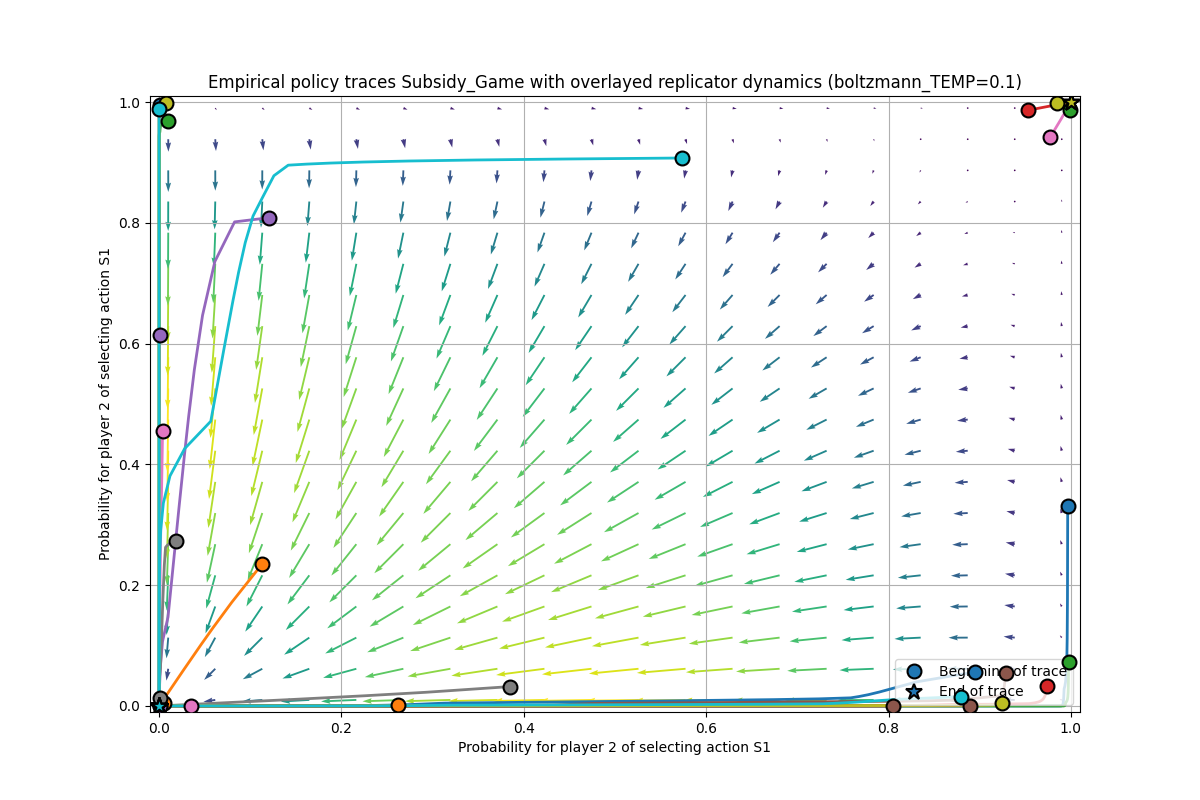
\includegraphics[width=\linewidth]{plots/replicator_trajectoreis_Subsidy_Game_boltzmann_TEMP=0.1.png}
            \caption{Subsidy Game}
        \end{subfigure}
        \hfill
        \begin{subfigure}{0.44\textwidth}
            \centering
            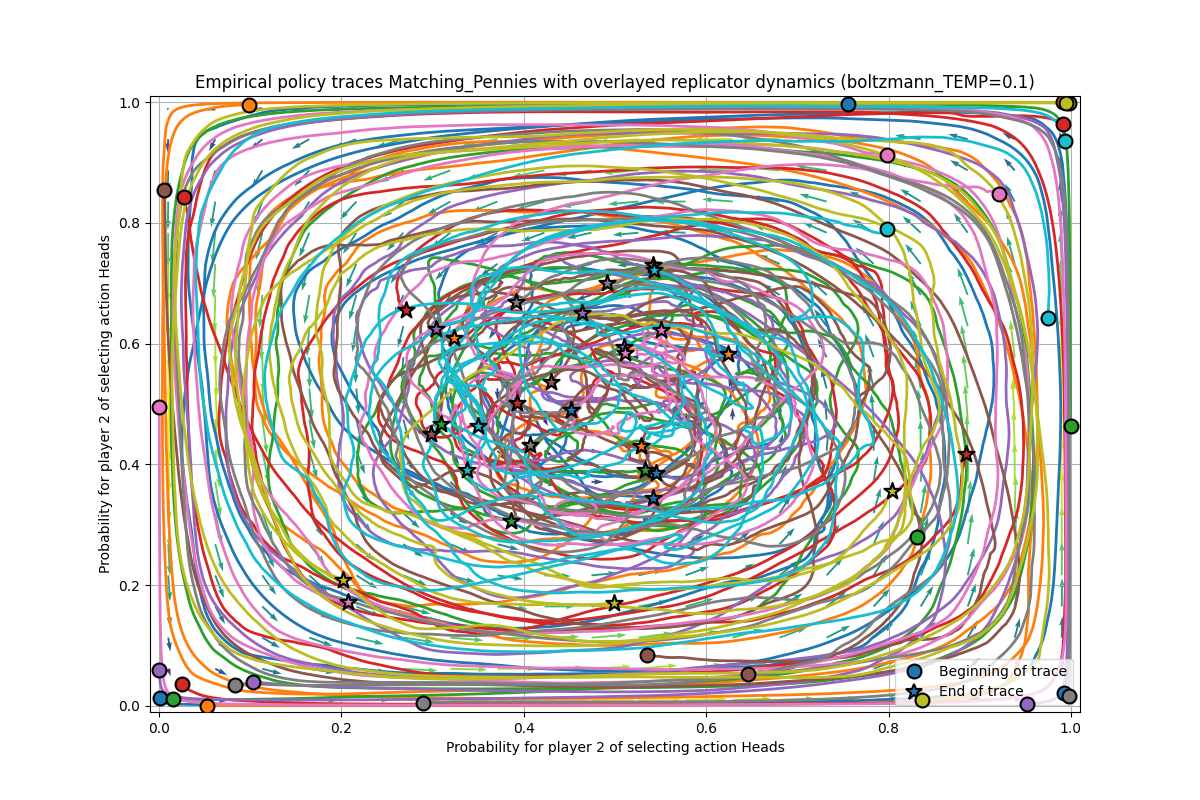
\includegraphics[width=\linewidth]{plots/replicator_trajectoreis_Matching_Pennies_boltzmann_TEMP=0.1.png}
            \caption{Matching Pennies}
        \end{subfigure}
        \caption{Empirical policy traces for Boltzmann Q-Learning (temperature = 0.1) across different games.}
        \label{fig:app_boltzmann_combined}
    \end{figure}

    \subsection{Lenient Boltzmann Q-Learning with Different K Values}

    \begin{figure}[H]
        \centering
        \begin{subfigure}{0.44\textwidth}
            \centering
            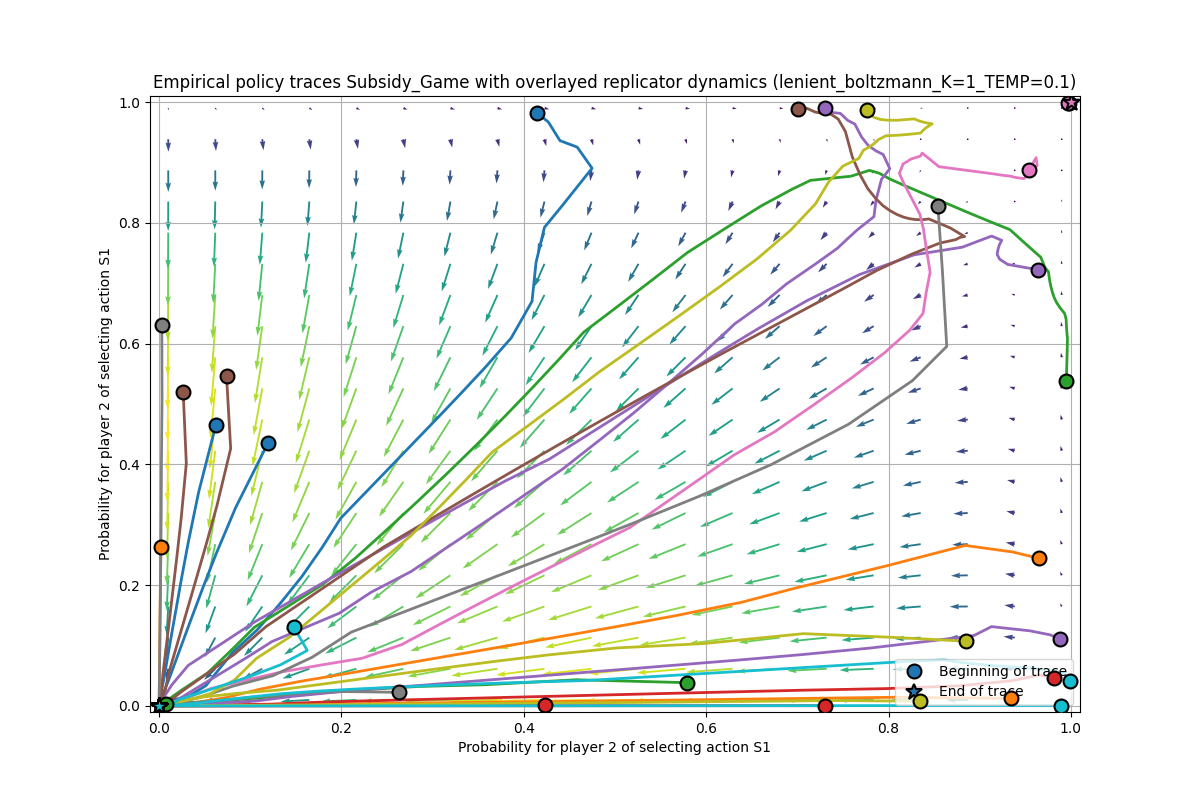
\includegraphics[width=\linewidth]{plots/replicator_trajectoreis_Subsidy_Game_lenient_boltzmann_K=1_TEMP=0.1.png}
            \caption{K=1}
        \end{subfigure}
        \hfill
        \begin{subfigure}{0.44\textwidth}
            \centering
            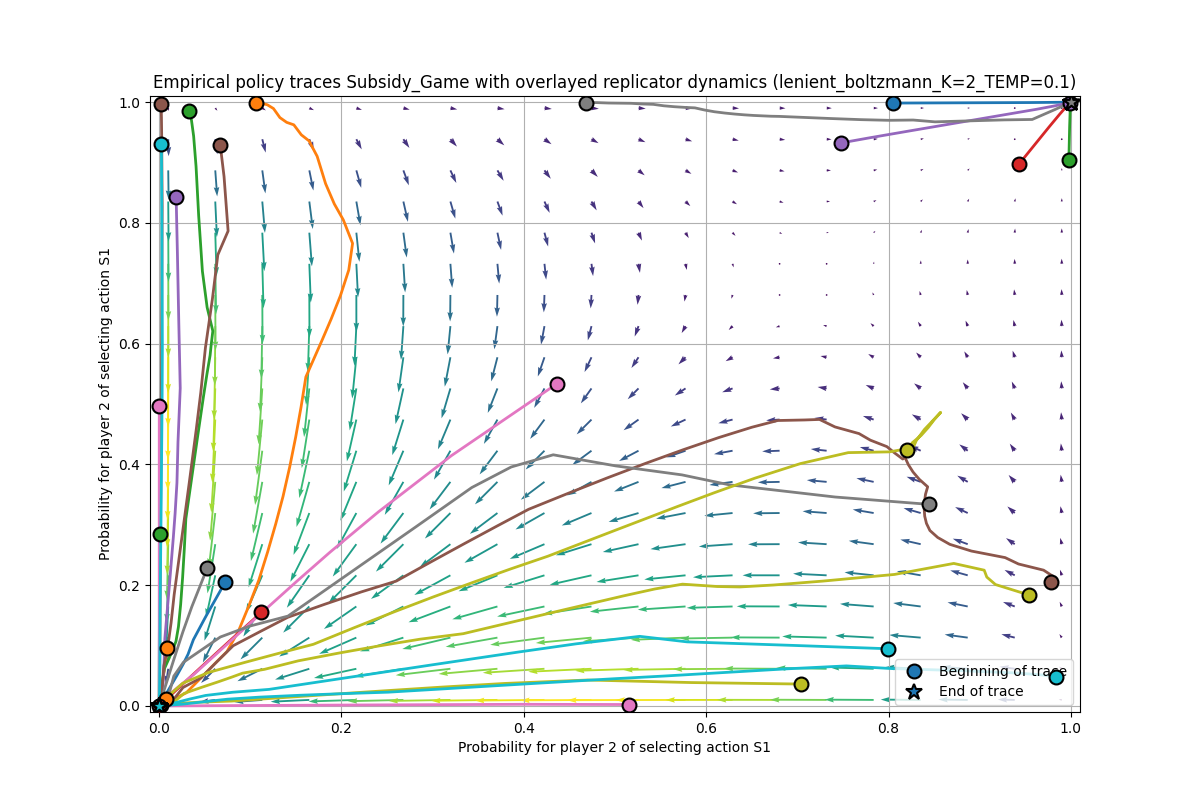
\includegraphics[width=\linewidth]{plots/replicator_trajectoreis_Subsidy_Game_lenient_boltzmann_K=2_TEMP=0.1.png}
            \caption{K=2}
        \end{subfigure}
        \vspace{0.5cm}
        \begin{subfigure}{0.44\textwidth}
            \centering
            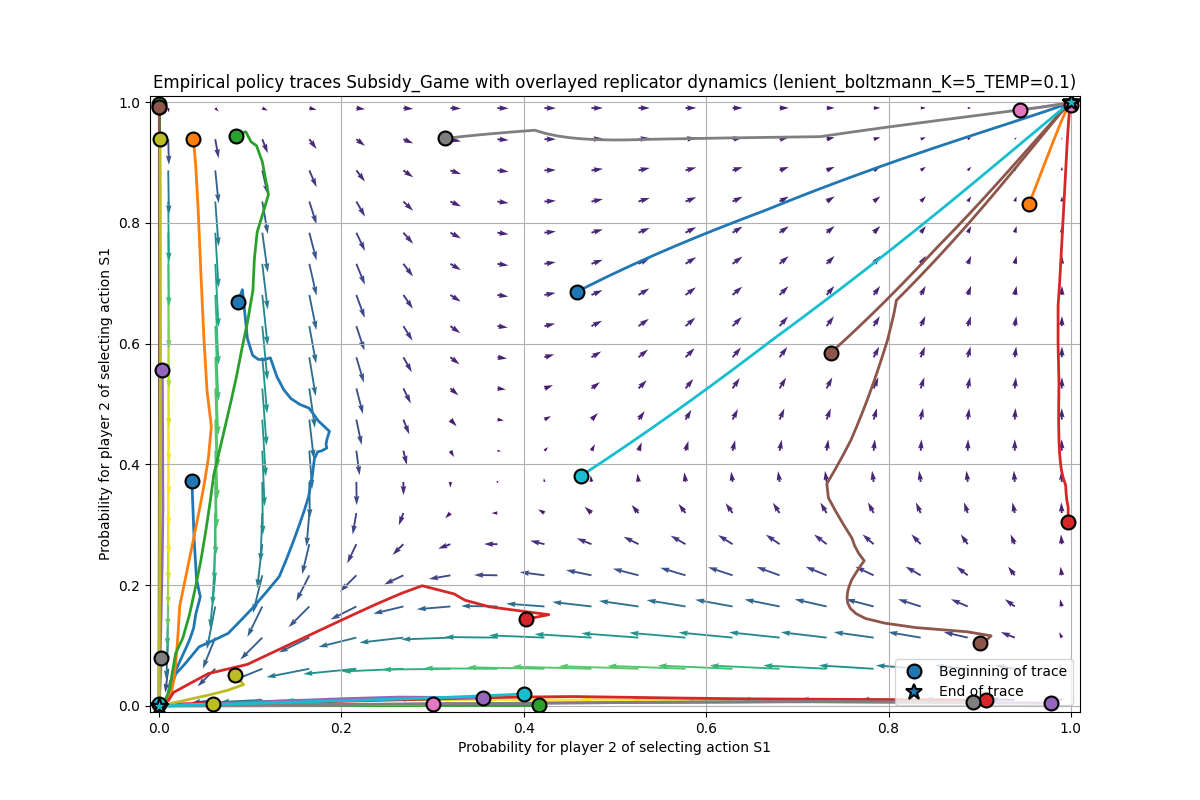
\includegraphics[width=\linewidth]{plots/replicator_trajectoreis_Subsidy_Game_lenient_boltzmann_K=5_TEMP=0.1.png}
            \caption{K=5}
        \end{subfigure}
        \hfill
        \begin{subfigure}{0.44\textwidth}
            \centering
            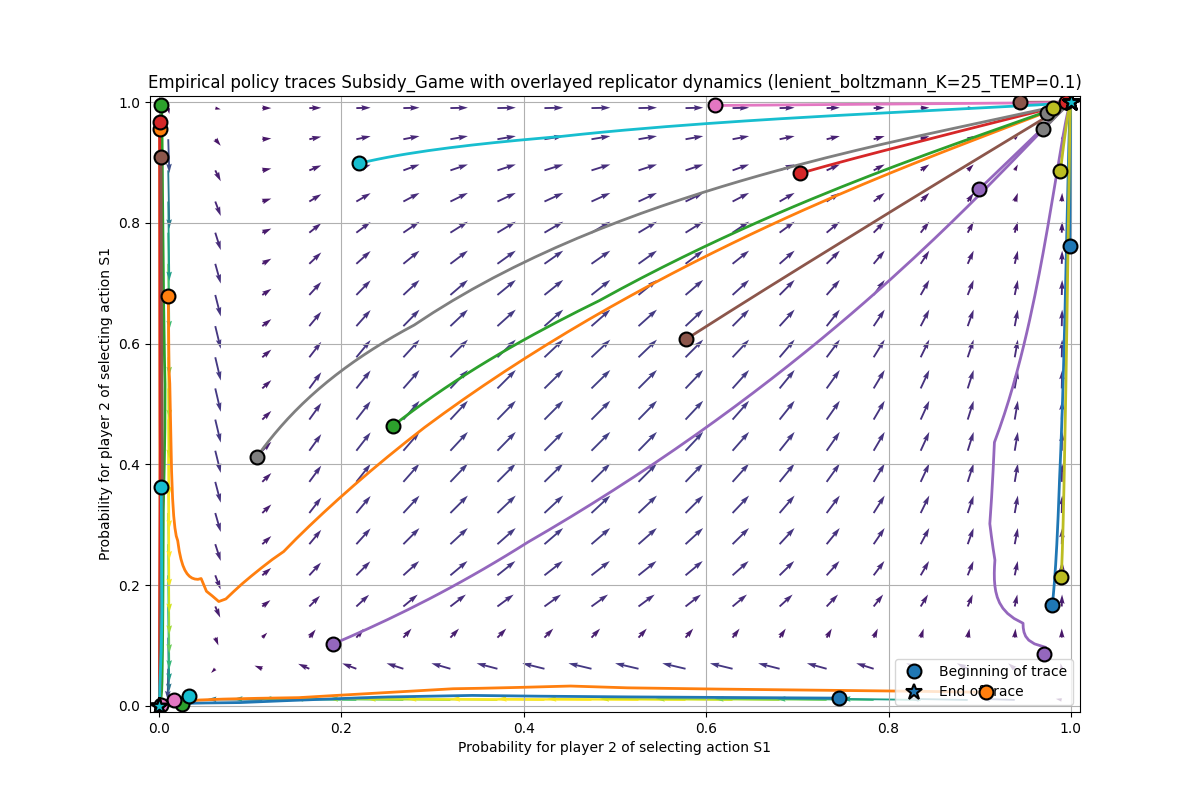
\includegraphics[width=\linewidth]{plots/replicator_trajectoreis_Subsidy_Game_lenient_boltzmann_K=25_TEMP=0.1.png}
            \caption{K=25}
        \end{subfigure}
        \caption{Empirical policy traces for Lenient Boltzmann Q-Learning on the Subsidy Game with different K values (temperature = 0.1).}
        \label{fig:app_subsidy_k_values}
    \end{figure}

    \begin{figure}[H]
        \centering
        \begin{subfigure}{0.44\textwidth}
            \centering
            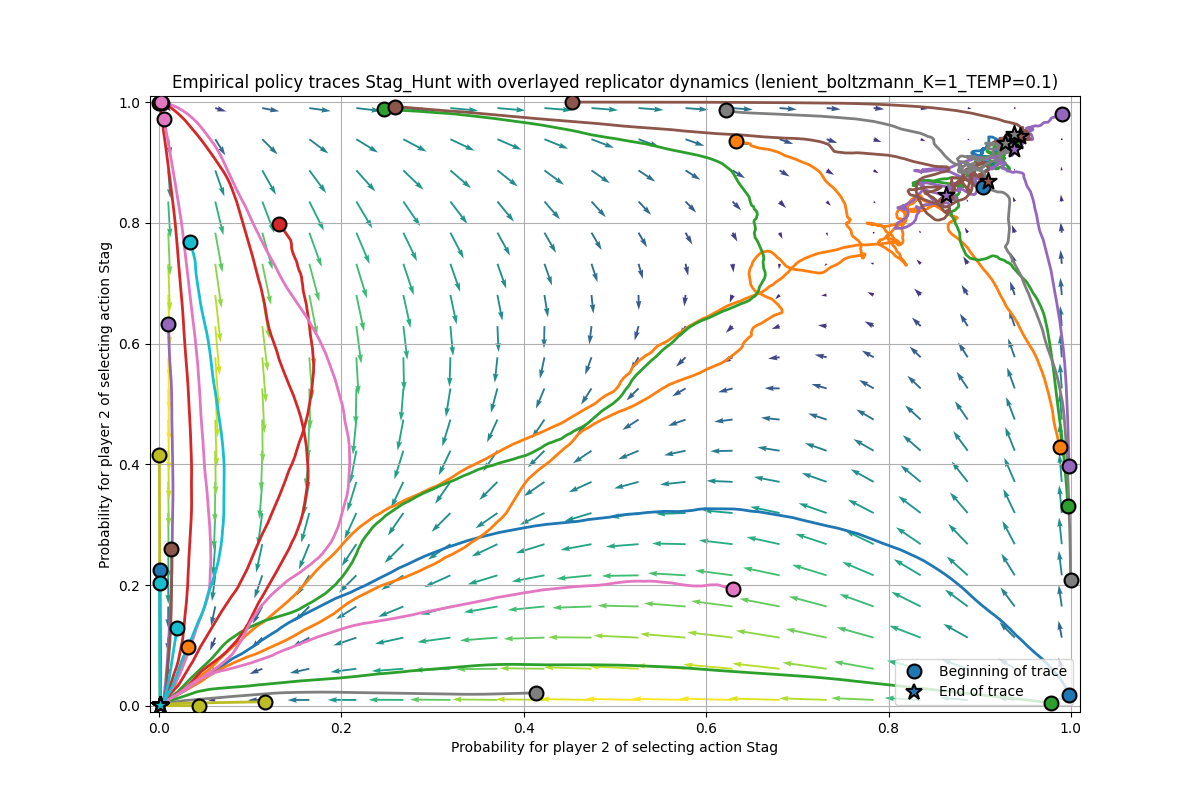
\includegraphics[width=\linewidth]{plots/replicator_trajectoreis_Stag_Hunt_lenient_boltzmann_K=1_TEMP=0.1.png}
            \caption{K=1}
        \end{subfigure}
        \hfill
        \begin{subfigure}{0.44\textwidth}
            \centering
            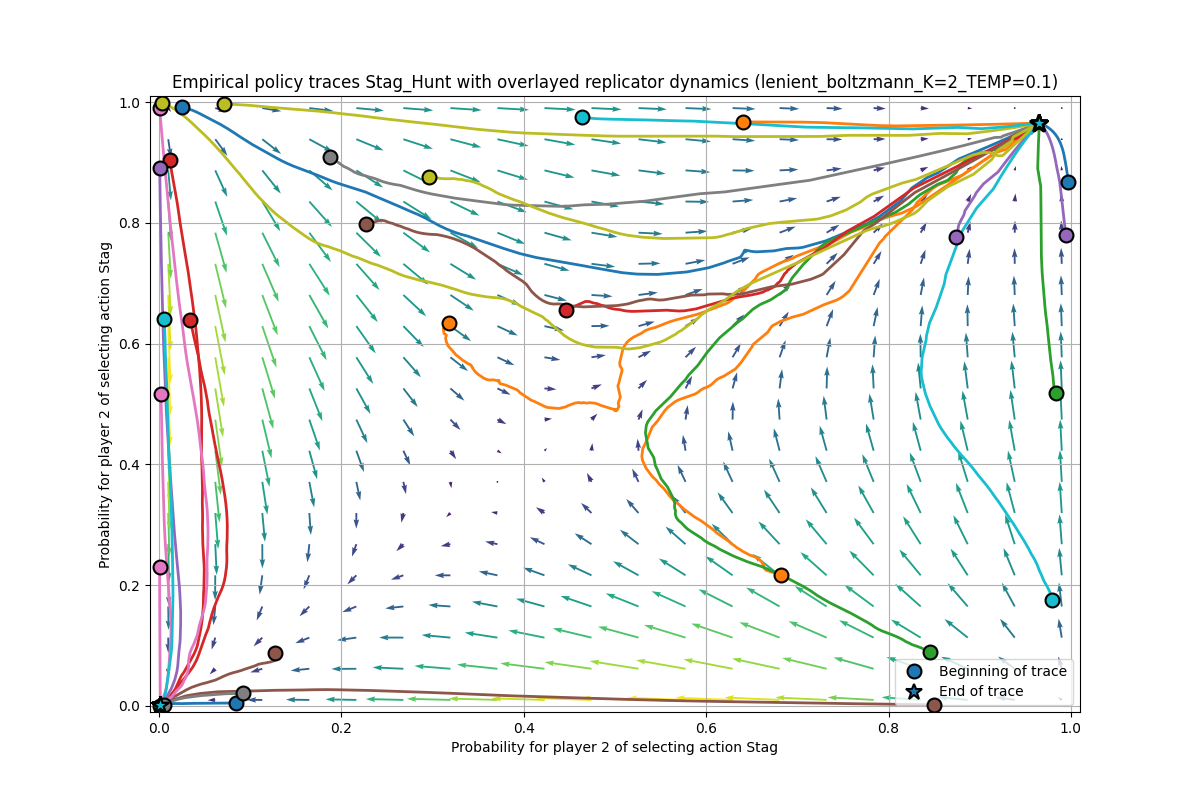
\includegraphics[width=\linewidth]{plots/replicator_trajectoreis_Stag_Hunt_lenient_boltzmann_K=2_TEMP=0.1.png}
            \caption{K=2}
        \end{subfigure}
        \vspace{0.5cm}
        \begin{subfigure}{0.44\textwidth}
            \centering
            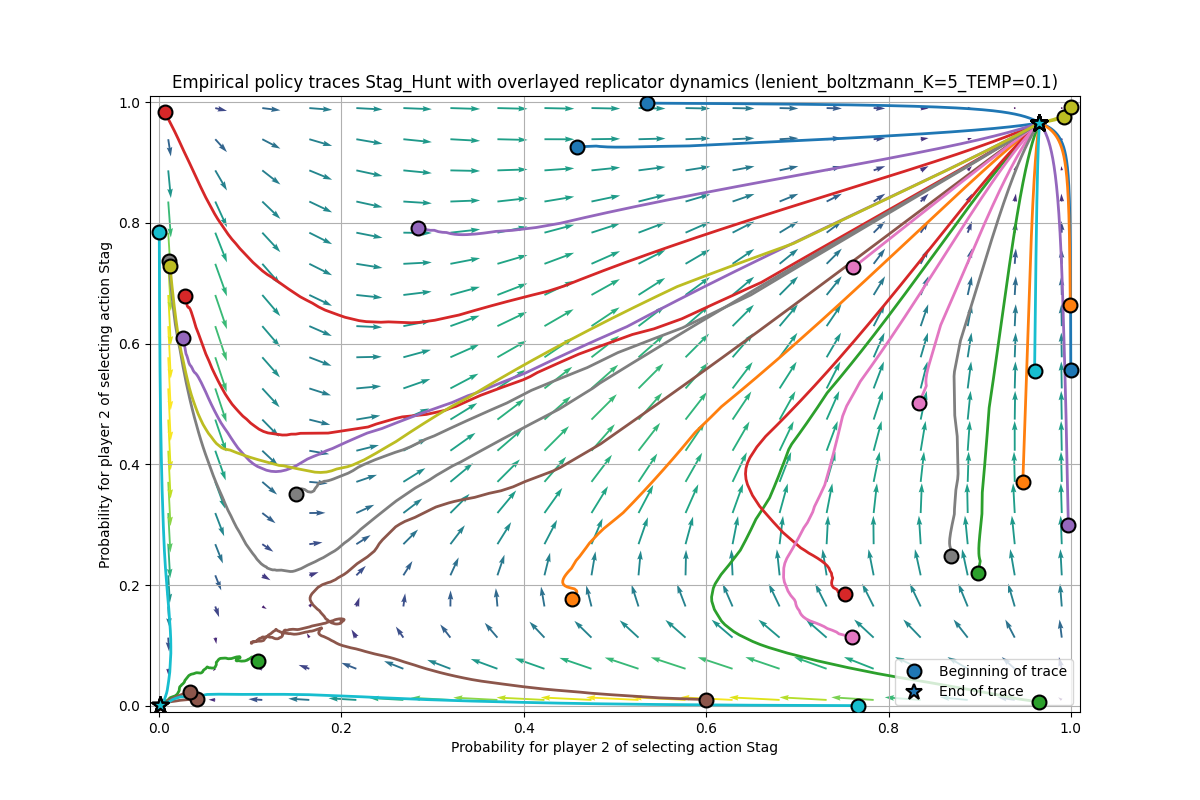
\includegraphics[width=\linewidth]{plots/replicator_trajectoreis_Stag_Hunt_lenient_boltzmann_K=5_TEMP=0.1.png}
            \caption{K=5}
        \end{subfigure}
        \hfill
        \begin{subfigure}{0.44\textwidth}
            \centering
            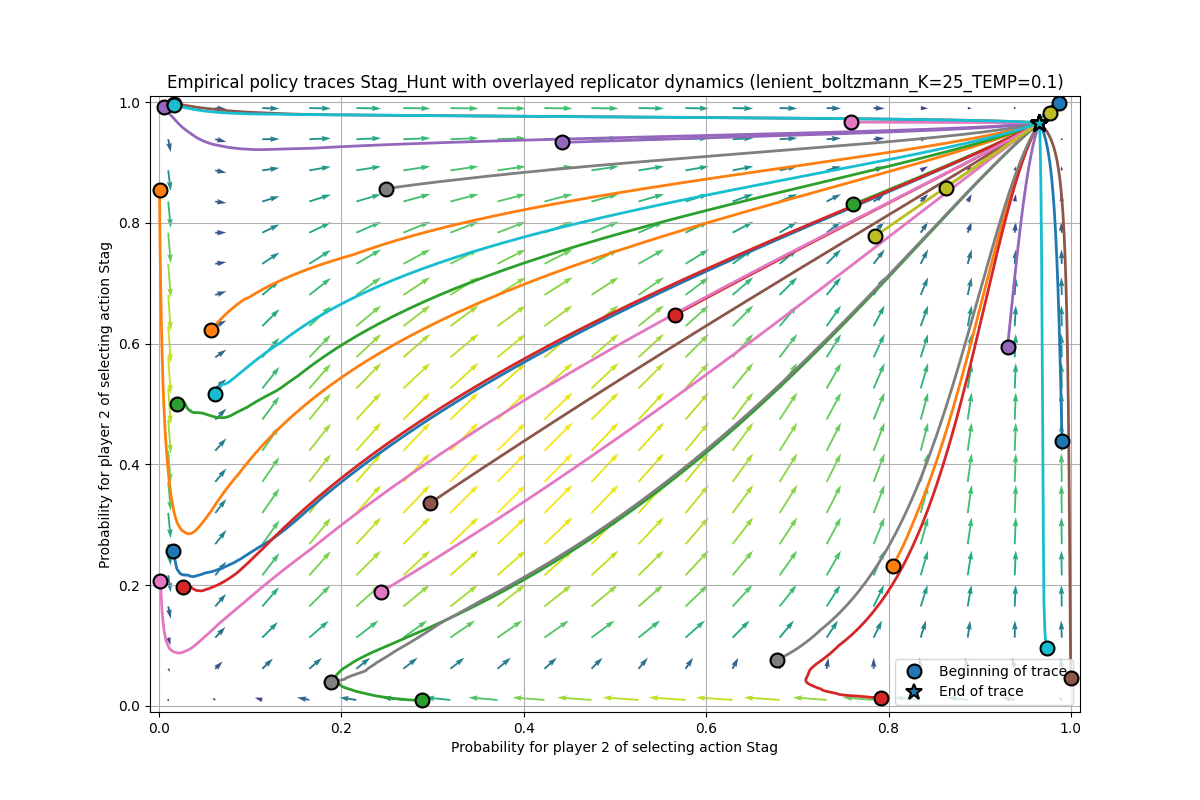
\includegraphics[width=\linewidth]{plots/replicator_trajectoreis_Stag_Hunt_lenient_boltzmann_K=25_TEMP=0.1.png}
            \caption{K=25}
        \end{subfigure}
        \caption{Empirical policy traces for Lenient Boltzmann Q-Learning on the Stag Hunt with different K values (temperature = 0.1).}
        \label{fig:app_stag_hunt_k_values}
    \end{figure}

    \begin{figure}[H]
        \centering
        \begin{subfigure}{0.44\textwidth}
            \centering
            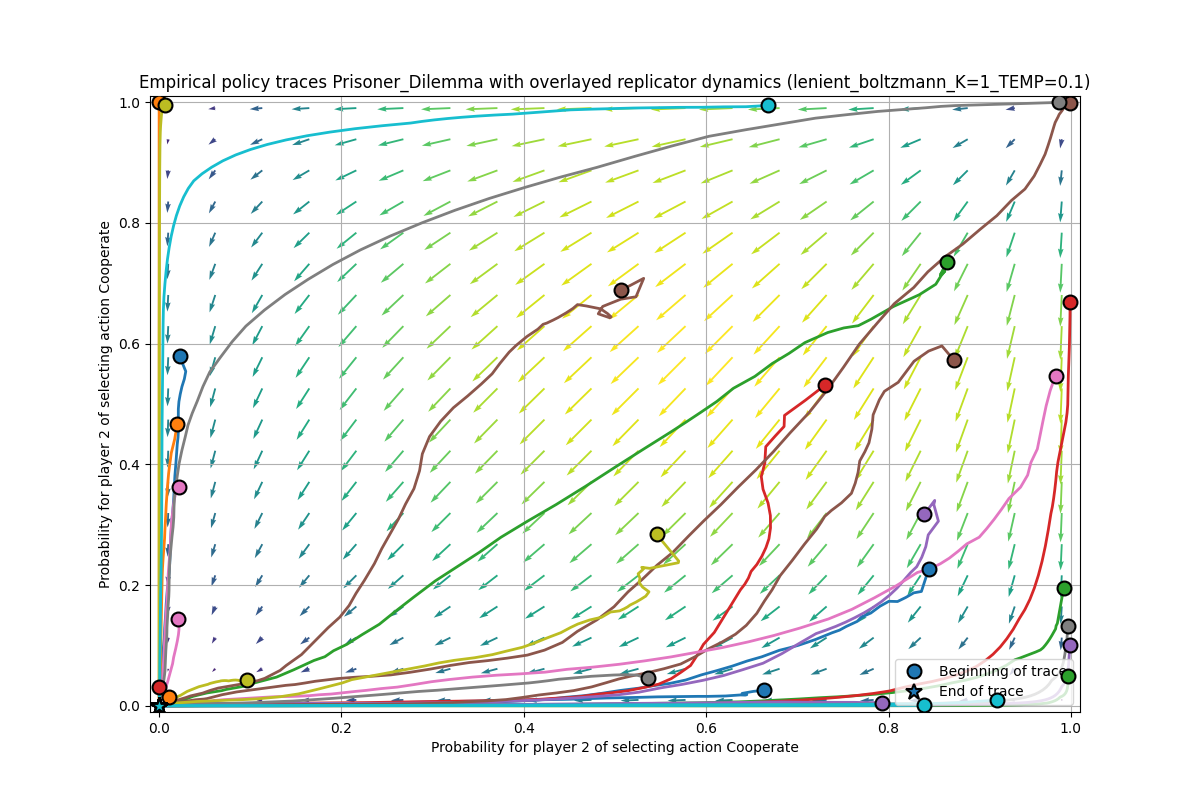
\includegraphics[width=\linewidth]{plots/replicator_trajectoreis_Prisoner_Dilemma_lenient_boltzmann_K=1_TEMP=0.1.png}
            \caption{K=1}
        \end{subfigure}
        \hfill
        \begin{subfigure}{0.44\textwidth}
            \centering
            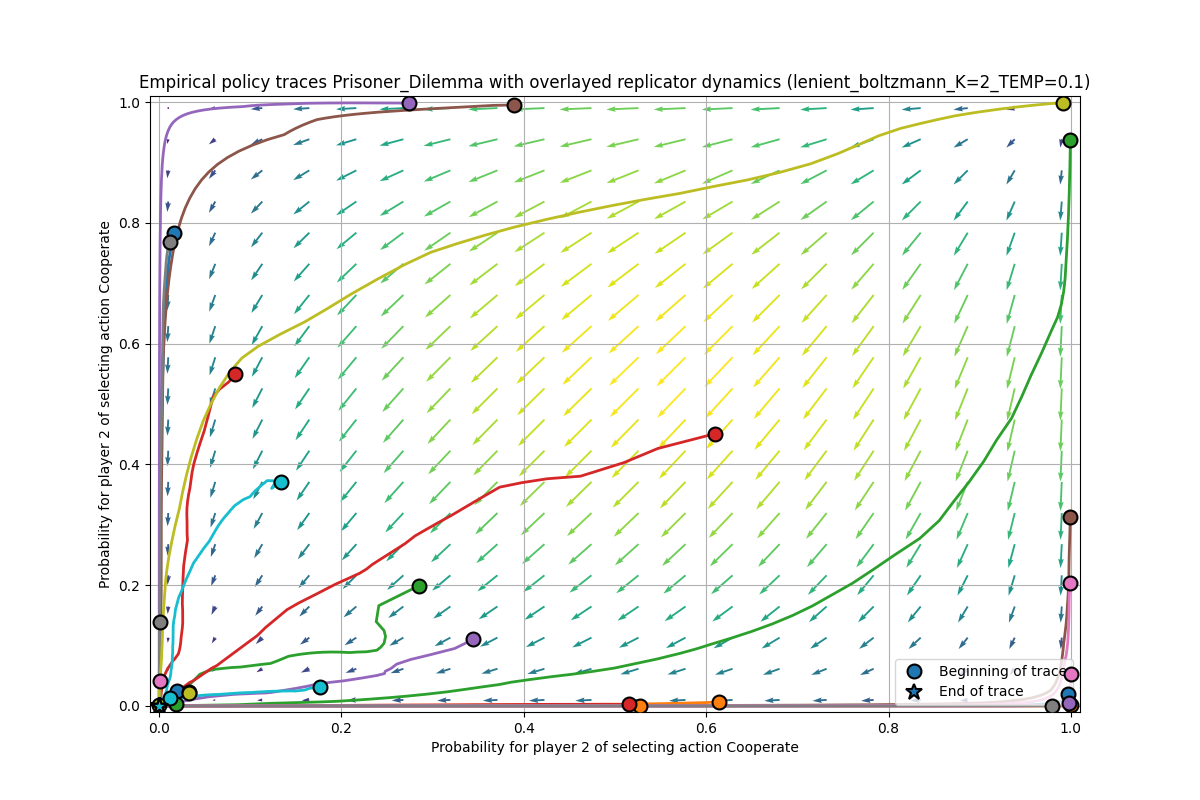
\includegraphics[width=\linewidth]{plots/replicator_trajectoreis_Prisoner_Dilemma_lenient_boltzmann_K=2_TEMP=0.1.png}
            \caption{K=2}
        \end{subfigure}
        \vspace{0.5cm}
        \begin{subfigure}{0.44\textwidth}
            \centering
            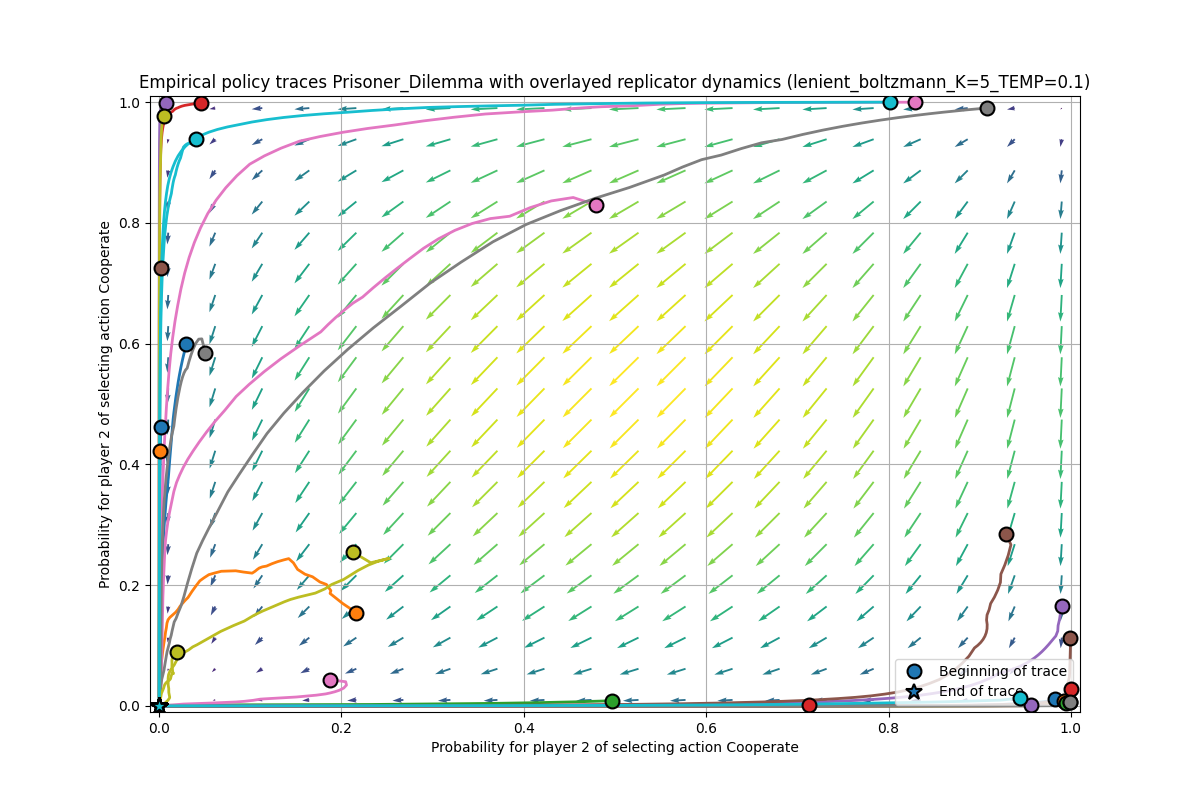
\includegraphics[width=\linewidth]{plots/replicator_trajectoreis_Prisoner_Dilemma_lenient_boltzmann_K=5_TEMP=0.1.png}
            \caption{K=5}
        \end{subfigure}
        \hfill
        \begin{subfigure}{0.44\textwidth}
            \centering
            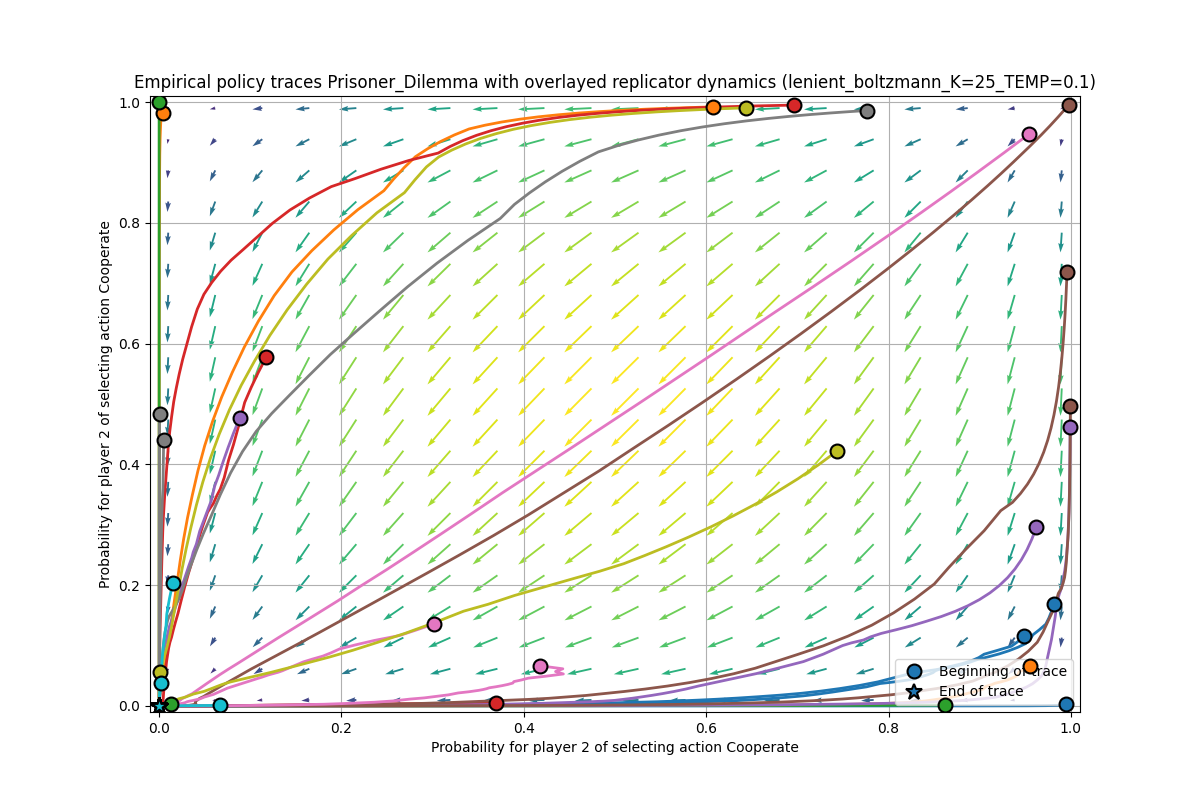
\includegraphics[width=\linewidth]{plots/replicator_trajectoreis_Prisoner_Dilemma_lenient_boltzmann_K=25_TEMP=0.1.png}
            \caption{K=25}
        \end{subfigure}
        \caption{Empirical policy traces for Lenient Boltzmann Q-Learning on the Prisoner's Dilemma with different K values (temperature = 0.1).}
        \label{fig:app_prisoner_k_values}
    \end{figure}

    \begin{figure}[H]
        \centering
        \begin{subfigure}{0.44\textwidth}
            \centering
            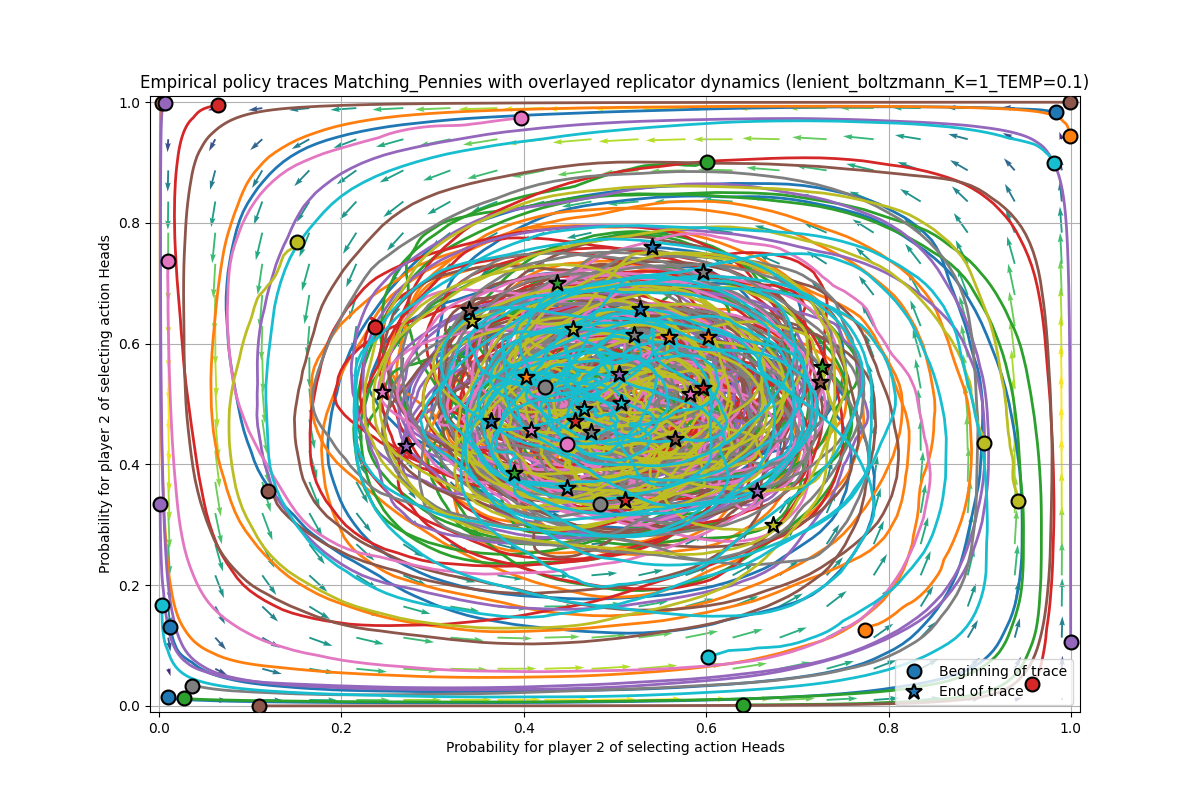
\includegraphics[width=\linewidth]{plots/replicator_trajectoreis_Matching_Pennies_lenient_boltzmann_K=1_TEMP=0.1.png}
            \caption{K=1}
        \end{subfigure}
        \hfill
        \begin{subfigure}{0.44\textwidth}
            \centering
            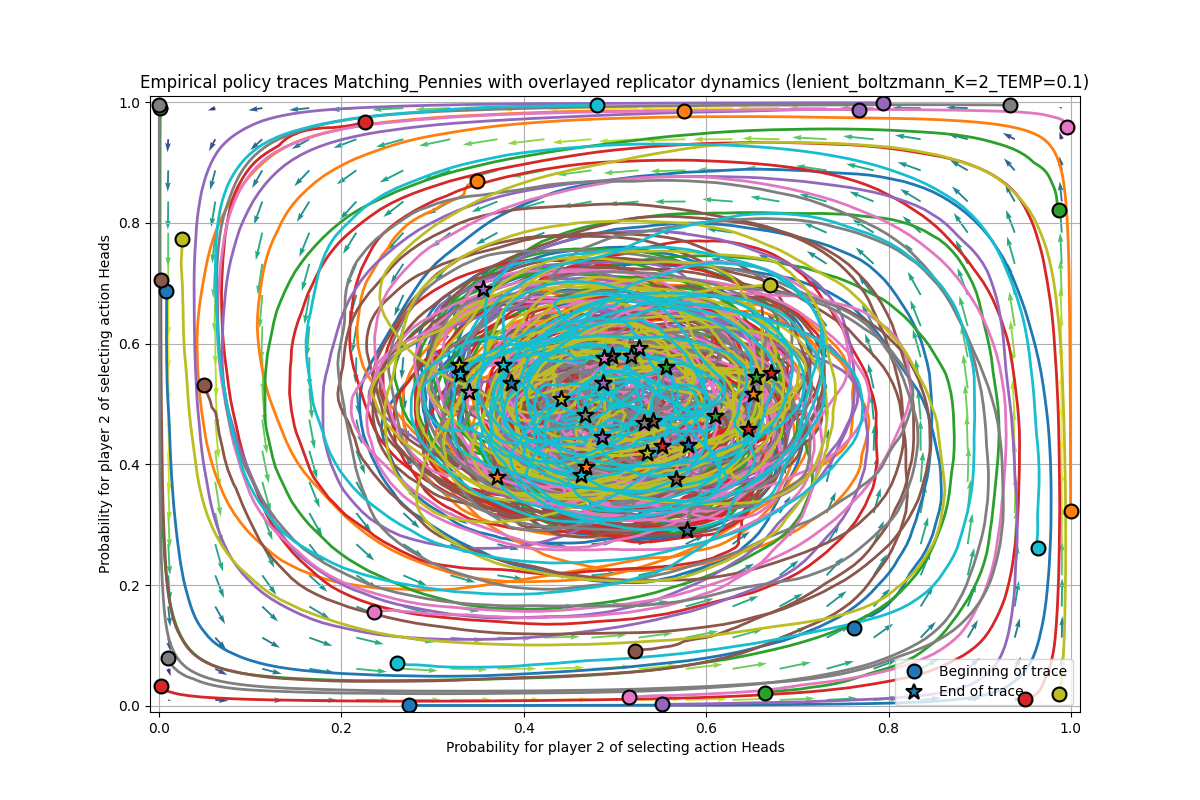
\includegraphics[width=\linewidth]{plots/replicator_trajectoreis_Matching_Pennies_lenient_boltzmann_K=2_TEMP=0.1.png}
            \caption{K=2}
        \end{subfigure}
        \vspace{0.5cm}
        \begin{subfigure}{0.44\textwidth}
            \centering
            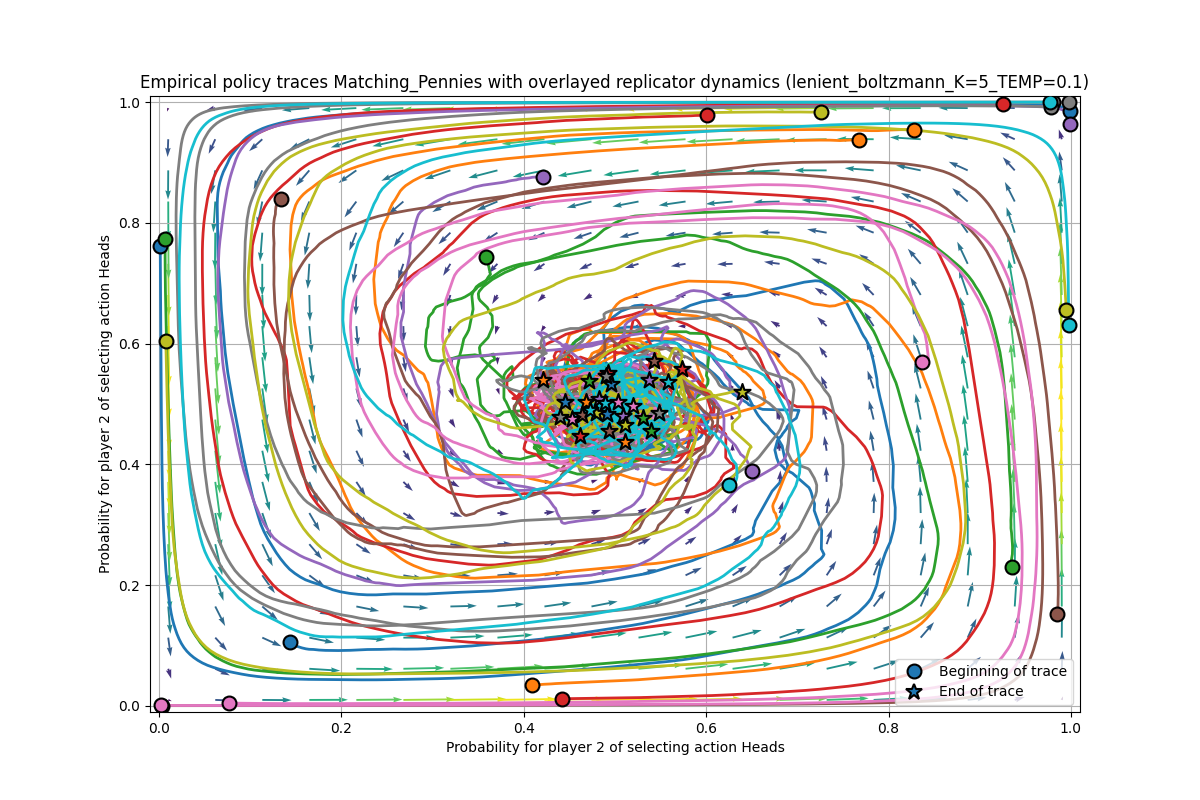
\includegraphics[width=\linewidth]{plots/replicator_trajectoreis_Matching_Pennies_lenient_boltzmann_K=5_TEMP=0.1.png}
            \caption{K=5}
        \end{subfigure}
        \hfill
        \begin{subfigure}{0.44\textwidth}
            \centering
            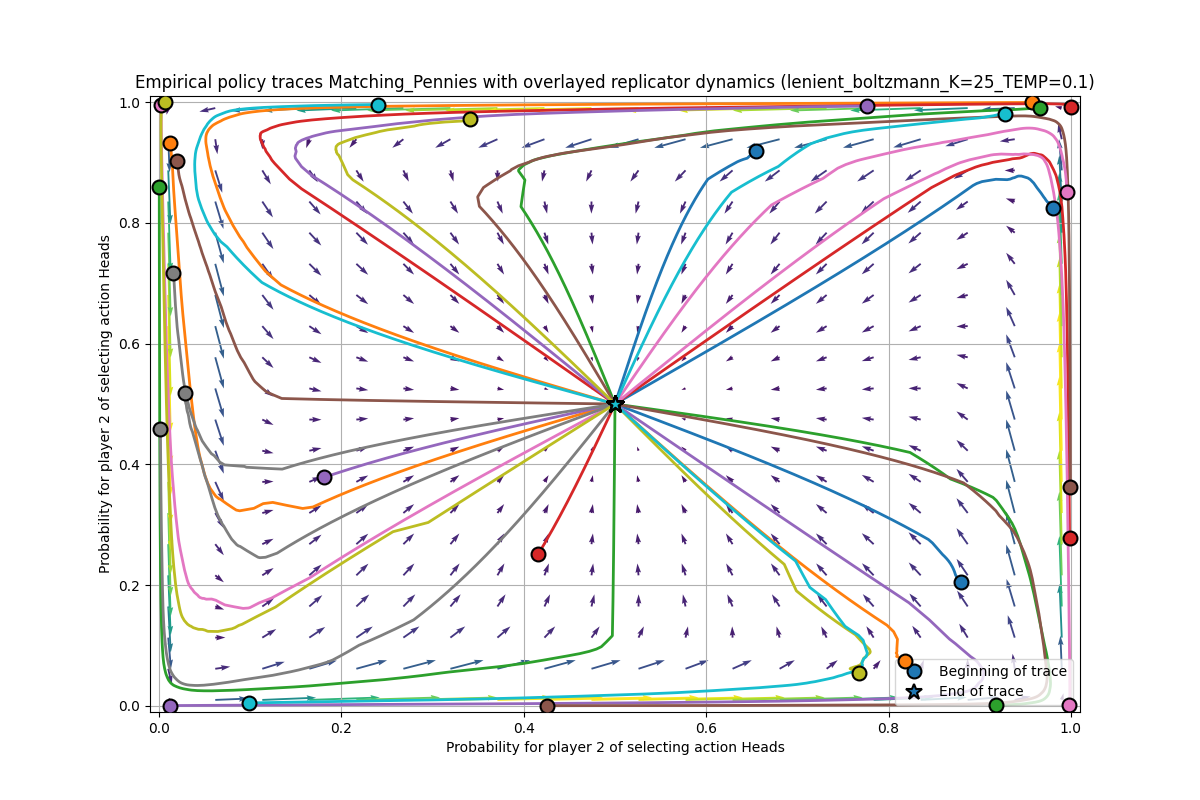
\includegraphics[width=\linewidth]{plots/replicator_trajectoreis_Matching_Pennies_lenient_boltzmann_K=25_TEMP=0.1.png}
            \caption{K=25}
        \end{subfigure}
        \caption{Empirical policy traces for Lenient Boltzmann Q-Learning on the Matching Pennies with different K values (temperature = 0.1).}
        \label{fig:app_matching_pennies_k_values}
    \end{figure}


    \section{Grid search hyperparameters and evaluation results}

    \begin{table}[H]
        \centering
        \begin{tabular}{|l|l|l|l|l|l|l|}
            \hline
            \textbf{Checkpoint}  & \textbf{Max Cycles} & \shortstack{\textbf{Rollout}
            \\\textbf{Length}} & \textbf{Arrows} & \textbf{KL} & \shortstack{\textbf{Score}\\\textbf{1000}} & \shortstack{\textbf{Score}\\\textbf{100000000}} \\
            \hline
            best\_977\_185.145   & 1000000             & 512                          & False & True  & 44.48 & 678.38 \\
            regular\_980\_184.05 & 1000000             & 512                          & False & True  & 44.24 & 446.56 \\
            regular\_980\_79.8   & 2000                & 512                          & True  & True  & 43.64 & 294.96 \\
            best\_915\_77.41     & 2000                & 512                          & True  & False & 43.26 & 194.82 \\
            best\_866\_72.985    & 2000                & 512                          & False & False & 42.0  & 151.16 \\
            regular\_980\_103.9  & 1000000             & 512                          & True  & True  & 41.46 & 194.70 \\
            regular\_980\_67.505 & 2000                & 512                          & False & True  & 41.36 & 167.72 \\
            regular\_980\_68.425 & 2000                & 512                          & True  & False & 41.2  & 249.12 \\
            best\_725\_183.565   & 1000000             & 512                          & True  & False & 39.96 & 91.56  \\
            regular\_980\_70.69  & 2000                & 512                          & False & False & 39.66 & 128.30 \\
            best\_905\_82.825    & 2000                & 512                          & True  & True  & 39.6  & 220.00 \\
            best\_992\_74.34     & 2000                & 512                          & False & True  & 38.02 & 131.32 \\
            regular\_980\_163.36 & 1000000             & 512                          & False & False & 36.98 & 169.16 \\
            regular\_980\_91.09  & 1000000             & 512                          & True  & False & 36.56 & 136.44 \\
            best\_741\_115.81    & 1000000             & 512                          & True  & True  & 34.88 & 116.34 \\
            best\_729\_190.635   & 1000000             & 512                          & False & False & 31.3  & 134.90 \\
            regular\_980\_39.005 & 1000000             & 256                          & True  & False & 29.22 & 51.42  \\
            best\_780\_33.735    & 2000                & 256                          & True  & True  & 26.56 & 36.06  \\
            regular\_980\_27.13  & 2000                & 256                          & True  & True  & 26.42 & 32.32  \\
            regular\_980\_36.28  & 1000000             & 256                          & True  & True  & 25.48 & 41.64  \\
            best\_694\_38.105    & 2000                & 256                          & True  & False & 24.52 & 36.12  \\
            regular\_980\_20.475 & 2000                & 256                          & False & False & 22.58 & 25.52  \\
            best\_919\_43.96     & 1000000             & 256                          & True  & True  & 21.76 & 30.30  \\
            regular\_980\_45.93  & 1000000             & 256                          & False & False & 21.34 & 22.28  \\
            regular\_980\_16.175 & 2000                & 256                          & False & True  & 21.02 & 25.06  \\
            regular\_980\_23.0   & 2000                & 256                          & True  & False & 21.0  & 38.78  \\
            best\_887\_51.605    & 1000000             & 256                          & True  & False & 20.9  & 22.70  \\
            best\_976\_45.825    & 1000000             & 256                          & False & False & 20.24 & 22.68  \\
            regular\_980\_26.575 & 1000000             & 256                          & False & True  & 17.62 & 18.42  \\
            best\_966\_27.86     & 1000000             & 256                          & False & True  & 17.5  & 19.02  \\
            best\_930\_28.79     & 2000                & 256                          & False & False & 16.68 & 20.08  \\
            best\_917\_23.735    & 2000                & 256                          & False & True  & 15.14 & 18.20  \\
            \hline
        \end{tabular}
        \caption{Evaluation results for different configurations for the PPO algorithm. All models were evaluated with 1000
            and 100000000 max cycles, and 50 different seeds. The checkpoint name description
            follows this format: whether it's a best score or a regular checkpoint, the epoch number and the score for that epoch. }
        \label{tab:app_best_models}
    \end{table}

    Notably, the scores obtained with 1000 and 100000000 max cycles do not exhibit a direct correlation.
    However, the score on 1000 remains a reliable indicator of policy quality, particularly for the top-performing models, while being faster to compute.
    The increased number of cycles helps to differentiate the best models among themselves.


    \section{Evaluation results for multi-agent PPO}

    \begin{table}[H]
        \centering
        \begin{tabular}{|l|l|l|l|}
            \hline
            \textbf{Checkpoint}         & \textbf{Modified Reward} & \shortstack{\textbf{Score}         \\\textbf{1000}} & \shortstack{\textbf{Score}\\\textbf{100000000}} \\
            \hline
            results\_46.3               & False                    & 43.5                       & 88.04 \\
            best\_101.16499999999999    & False                    & 17.3                       & 40.52 \\
            best\_311.43                & True                     & 41.52                      & 98.78 \\
            results\_291.70000000000005 & True                     & 35.7                       & 84.84 \\
            \hline
        \end{tabular}
        \caption{Evaluation results for multi-agent PPO.}
        \label{tab:multi_ppo_results}
    \end{table}
    Using modified reward schema seems to improve agents final score. It's worth to point out that, it might be possible
    that there exists some earlier checkpoint which might have flipped the results, but we do not have time nor resources
    to test all the checkpoints.

\end{appendices}


\end{document}